% ????
% TO DO: 
% Include description of how to visualize MSAs using hhfilter and reformat!

%\documentclass[final,1p,times]{elsarticle}
\documentclass[11pt,a4paper]{article}
\usepackage{url}
\usepackage{cite}
\usepackage{longtable}
\usepackage{graphicx}
\usepackage{amsmath}
\usepackage{fancyvrb}

\setlength{\parindent}{0mm}
\setlength{\oddsidemargin}{-2mm}
\setlength{\oddsidemargin}{-2mm}
\setlength{\topmargin}{0mm}
\setlength{\textheight}{245mm}
\setlength{\textwidth}{165mm}
\setlength{\headheight}{0mm}
\setlength{\headsep}{0mm}
\setlength{\parskip}{3mm}

\usepackage{bookmark,hyperref}

\hypersetup{
%     bookmarks=true,         % show bookmarks bar?
    unicode=true,          % non-Latin characters in Acrobat’s bookmarks
    pdftoolbar=true,        % show Acrobat’s toolbar?
    pdfmenubar=true,        % show Acrobat’s menu?
    pdffitwindow=false,     % window fit to page when opened
    pdfstartview={FitH},    % fits the width of the page to the window
    pdftitle={HHsuite User Guide},      % title
    pdfauthor={Johannes S\"oding},  % author
    pdfsubject={HHsuite for sensitive sequence searching based on HMM-HMM alignment},   % subject of the document
    pdfnewwindow=true,      % links in new window
    colorlinks=true,        % false: boxed links; true: colored links
    linkcolor=black,        % color of internal links
    citecolor=black,        % color of links to bibliography
%     filecolor=black,        % color of file links
%     urlcolor=black,         % color of external links
}
%\urlstyle{same}            % show urls using the same font as the text

\newcommand{\hhversion}{Version 3.0.0, March 2015} 

%\title{HHsuite for sensitive sequence searching\\[2mm] based on HMM-HMM alignment} 

\begin{document}
\bibliographystyle{unsrt}
%\maketitle

\begin{center}

\vspace{20mm}
 
{\huge \bf HHsuite for sensitive protein sequence\\[2mm] searching based on HMM-HMM alignment}\\[4mm] 

{\Large \bf User Guide}

  \hhversion\\[2mm]
{\copyright  Johannes S\"oding, Markus Meier, Martin Steinegger, Michael Remmert, Andreas Hauser, Christof Angerm\"uller, Armin Meier and Andreas Biegert}\\[2mm]\


{\bf \Large Summary}

\end{center}

\noindent The HHsuite is an open-source software package for sensitive protein sequence searching based on the pairwise alignment of hidden Markov models (HMMs). It contains HHsearch [1] and HHblits [2] among other programs and utilities. HHsearch takes as input a multiple sequence alignment (MSA) or profile HMM and searches a database of HMMs (e.g.\ PDB, Pfam, or InterPro) for homologous proteins. HHsearch is often used for protein structure prediction to detect homologous templates and to build highly accurate query-template pairwise alignments for homology modeling. In the CASP9 competition (2010), a fully automated version of HHpred based on HHsearch and HHblits was ranked best out of 81 servers in template-based structure prediction. HHblits can build high-quality MSAs starting from single sequences or from MSAs. It transforms these into a query HMM and iteratively searches through uniprot20 database by adding significantly similar sequences from the previous search to the updated query HMM for the next search iteration. Compared to PSI-BLAST, HHblits is faster, up to twice as sensitive and produces more accurate alignments. HHblits uses the same HMM-HMM alignment algorithms as HHsearch, but it employs a fast prefilter that reduces the number of database HMMs for which to perform the slow HMM-HMM comparison from tens of millions to a few thousands. 
\\[2mm]

{\bf References:}


\begin{tabular}[t]{ll}
[1] & S\"oding J. (2005)\\ 
    & Protein homology detection by HMM-HMM comparison.\\
    & {\it Bioinformatics} {\bf 21}, 951-960.\\[2mm]

[2] & Remmert M., Biegert A., Hauser A., and S\"oding J. (2011) \\
    & HHblits: Lightning-fast iterative protein sequence searching by HMM-HMM alignment. \\
    & {\it Nat.\  Methods} {\bf 9}, 173-175.\\
\end{tabular}



\newpage

\setlength{\parskip}{0mm}
\tableofcontents
\setlength{\parskip}{2mm}

\newpage

\section{Introduction}
The HHsuite is an open-source software package for highly sensitive sequence searching and sequence alignment. Its two most important programs are HHsearch and HHblits. Both are based on the pairwise comparison of \textit{profile hidden Markov models} (HMMs). 

Profile HMMs are a concise representation of \textit{multiple sequence alignments} (MSAs) \cite{Durbin:2008,Krogh:1994}. Like sequence profiles, they contain for each position in the master sequence the probabilities to observe each of the 20 amino acids in homologous proteins. The amino acid distributions for each column are extrapolated from the homologous sequences in the MSA by adding \textit{pseudocounts} to the amino acid counts observed in the MSA. Unlike sequence profiles, profile HMMs also contain position-specific gap penalties. More precisely, they contain for each position in the master sequence the probability to observe an insertion or a deletion after that position (the log of which corresponds to gap-open penalties) and the probabilities to extend the insertion or deletion (the log of which corresponds to gap-extend penalties). A profile HMM is thus much better suited than a single sequence to find homologous sequences and calculate accurate alignments. By representing both the query sequence and the database sequences by profile HMMs, HHsearch and HHblits are more sensitive for detecting and aligning remotely homologous proteins than methods based on pairwise sequence comparison or profile-sequence comparison.

HHblits can build high-quality multiple sequence alignments (MSAs) starting from a single sequence or from an MSA. Compared to PSI-BLAST \cite{Altschul:1997}, HHblits is faster, finds up to two times more homologous proteins and produces more accurate alignments. It uses an iterative search strategy, adding sequences from significantly similar database HMMs from a previous search iteration to the query HMM for the next search. Because HHblits is based on the pairwise alignment of profile HMMs, it needs its own type of databases that contain multiple sequence alignments and the corresponding profile HMMs instead of single sequences. The HHsuite database uniprot20 is generated regularly by clustering the UniProt database \cite{uniprot:2010} from EBI/SIB/PIR and the nonredundant (nr) database from the NCBI into groups of similar sequences alignable over at least 80 \% of their length and down to $\sim 20 \%$ pairwise sequence identity. This database can be downloaded together with HHblits. HHblits uses the HMM-HMM alignment algorithms in HHsearch, but it employs a fast prefilter (based partly on code from Michael Farrar, \cite{Farrar:2007}) that reduces the number of database HMMs for which to perform the slow HMM-HMM comparison from tens of millions to a few thousands. At the same time, the prefilter is sensitive enough to reduce the sensitivity of HHblits only marginally in comparison to HHsearch. 

By generating highly accurate and diverse MSAs, HHblits can improve almost all downstream sequence analysis methods, such as the prediction of secondary and tertiary structure \cite{Jones:1999, Marks:2011}, of membrane helices, functionally conserved residues, binding pockets, protein interaction interfaces, or short linear motifs. The accuracy of all these methods depends critically on the accuracy and the diversity of the underlying MSAs, as too few or too similar sequences do not add significant information for the predictions. As an example, running the popular PSIPRED secondary structure prediction program \cite{Jones:1999} on MSAs generated by HHblits instead of PSI-BLAST improved the accuracy of PSIPRED significantly even without retraining PSIPRED on the HHblits alignments \cite{Remmert:2011}. 

HHsearch takes as input an MSA (e.g.\ built by HHblits) or a profile HMM and searches a database of HMMs for homologous proteins. The pdb70 database, for instance, consists of profile HMMs for a set of representative sequences from the PDB database \cite{PDB:2004}; the scop70 database has profile HMMs for representative domain sequences from the SCOP database of structural domains \cite{SCOP:2000}; the Pfam \cite{Finn:2010} domain database is a large collection of curated MSAs and profile HMMs for conserved, functionally annotated domains. HHsearch is often used to predict the domain architectures and the functions of domains in proteins by finding similarities to domains in the pdb70, Pfam or other databases. 

In addition to the command line package described here, the interactive web server at \url{http://hhpred.tuebingen.mpg.de} \cite{Soding:2005b, Hildebrand:2009} run HHsearch and HHblits. It offers extended functionality, such as Jalview applets for checking query and template alignments, histogram views of alignments, and building 3D models with MODELLER \cite{Sali:1993}. 

In the CASP9 competition (Critical Assessment of Techniques for Protein Structure Prediction) in 2010, a fully automated version of HHpred based on HHsearch and HHblits was ranked best out of the 81 servers in template-based structure prediction, the category most relevant for biological applications, while having an average response time of minutes instead of days like most other servers \cite{Mariani:2011} (\url{http://predictioncenter.org/casp9/groups_analysis.cgi?type=server&tbm=on}). 

Other popular programs for sensitive, iterative protein sequence searching are PSI-BLAST \cite{Altschul:1997} and HMMER (\url{http://hmmer.org/}). Since they are based on profile-to-sequence and HMM-to-sequence comparison, respectively, they have the advantage over HHblits and HHsearch of being able to search raw sequence databases.


\section{Installation of the HHsuite and its databases}

The HHsuite source code, executable RPM and DPKG packages for most Linux 64 bit platforms, MAC OS X, and BSD Unix, utility scripts in Perl/Python:
\begin{verbatim}
  https://github.com/soedinglab/HHsuite
\end{verbatim}


Databases can be downloaded at:
\begin{verbatim}
  http://wwwuser.gwdg.de/~compbiol/data/hhsuite/databases/hhsuite_dbs/
\end{verbatim}

\subsection{Supported platforms and hardware requirements} \label{installation}

HHsuite needs a 64 bit system to read files larger than 4 GB. HHsuite has been extensively tested on 64 bit Linux, in particular Arch Linux, Debian, Ubuntu, Scientific Linux (SL), and Red Hat. We have done limited testing under BSD, MAX OS X, and CygWin. We plan to offer a 64 bit Windows version compiled under MinGW in the future.

HHsuite typically requires at least 4GB of main memory. Memory requirements can be estimated as follows:
%\textrm{Memory req.} = \textrm{Query\_length} \times \textrm{max\_db\_seq\_length} \times \textrm{num\_threads} \times (4 (SSE) or 8 (AVX2)) \trextrm{B} + \textrm{Query\_length} \times \textrm{max\_db\_seq\_length} \times \textrm{num\_threads} \times 8 \trextrm{B} + 1 \textrm{GB} 

\begin{equation}
\begin{split}
\textrm{Memory req.} & = \textrm{query\_length} \times \textrm{max\_db\_seq\_length} \times \textrm{num\_threads} \times \textrm{(4 (SSE) or 8 (AVX2))} \textrm{B} \\
 & + \textrm{query\_length} \times \textrm{max\_db\_seq\_length} \times \textrm{num\_threads} \times 8 \textrm{B} + 1 \textrm{GB} 
\end{split}
\end{equation}
Here, num\_threads is the number of threads specified with option \verb`-cpu <int>`.

Due to the high number of random file accesses by HHblits, it is important for good efficiency that the databases used by HHblits are placed in RAM disk or on a local solid state drive (SSD). See section \ref{efficiency} for details.


\subsubsection*{Support for SSSE3 instruction set} 

HHblits needs to run on CPUs supporting at least the SSSE3 (Supplemental Streaming SIMD Extensions 3) instruction set. (See \url{https://en.wikipedia.org/wiki/SSSE3} for an explanation of SSSE3.) Starting with the Woodcrest Xeons in 2006, all Intel CPUs support SSSE3. By default, the HHsuite binaries are compiled using the most evolved supported instruction set on the computer used for compiling.

However, you may limit the used instruction set to SSSE3 with the cmake compile flag \verb`-DHAVE_SSSE3=1`
The precompiled standard binaries are compiled with this flag. 

\subsection{Installation from source code} 

\newcounter{mycounter}  
\newenvironment{enum}
 {\begin{list}{\arabic{mycounter}.~~}{\usecounter{mycounter} \labelsep=0em \labelwidth=0em \leftmargin=0em \itemindent=0em}}
 {\end{list}}


\begin{enum}

\item Download the sources from \url{https://github.com/soedinglab/hh-suite/releases}, for example
\begin{verbatim}
$ mkdir ~/programs/hh/
$ cd ~/programs/hh/
$ wget https://github.com/soedinglab/hh-suite/releases/.../hhsuite-3.0-beta.1-Source.tar.gz 
\end{verbatim}
\vspace{2mm}


\item Then unzip and untar the file
\begin{verbatim}
$ tar -xzvf hhsuite-3.0-beta.1-Source.tar.gz
\end{verbatim}
This will unpack the sources to \verb`hhsuite-<VERSION>`.
\vspace{2mm}


\item Compilation: Run make in the source directory:
\begin{verbatim}
$ cd hhsuite-<VERSION>/
$ mkdir build
$ cd build
$ cmake -DCMAKE_BUILD_TYPE=RelWithDebInfo -G "Unix Makefiles" \\
    -DCMAKE_INSTALL_PREFIX=${INSTALL_BASE_DIR} ..
$ make
$ make install
\end{verbatim}

Set \verb`${INSTALL_BASE_DIR}` to the absolute path of the base directory where you want install HHsuite.
For example, to install into \verb`/usr/local/hhsuite`:
\begin{verbatim}
$ cmake -DCMAKE_BUILD_TYPE=RelWithDebInfo -G "Unix Makefiles" \\
    -DCMAKE_INSTALL_PREFIX=/usr/local/hhsuite ..
\end{verbatim}

The HHsuite binaries will then be put into \verb`/usr/local/hhsuite/bin`.

\vspace{2mm}

\item Set HHLIB and paths: In your shell, set the environment variable HHLIB to \verb`${INSTALL_BASE_DIR}`, 
e.g, for bash, zsh, or ksh,
\begin{verbatim}
$ export HHLIB=${INSTALL_BASE_DIR}
\end{verbatim}
and, for csh or tcsh: \verb`$ setenv HHLIB=${INSTALL_BASE_DIR}`. 
HHsearch and HHblits look for the column state library file \verb`cs219.lib`
and the context library file \verb`context_data.crf` in \verb`$HHLIB/data/`. The HHsuite
python/perl scripts also read HHLIB (via file \verb`scripts/HHPaths.pm`) to locate HHsuite binaries and data files.

Put the location of your HHsuite binaries and scripts into your search path:
\begin{verbatim}
$ export PATH=$PATH:$HHLIB/bin:$HHLIB/scripts
\end{verbatim}

To avoid typing these commands every time you open a new shell, you may add the following lines to the \verb`.bashrc`, \verb`.kshrc`, \verb`.cshrc` or equivalent file in your home directory that is executed every time a shell is started:
\begin{verbatim}
export HHLIB=/usr/local/
PATH=$PATH:$HHLIB/bin>:$HHLIB/scripts
alias hhblits='hhblits -d <path_to/uniprot20>'
\end{verbatim}
The last line defines a default database for hhblits. 
\vspace{2mm}

\end{enum}

\subsection{Package installation}

\subsubsection*{Installation under x86 64bit Linux with the red hat package manager RPM}

If you use a RPM based distribution like Scientific Linux (SL), Red Hat Enterprise Linux (RHEL) or CentOS we provide precompiled x86\_64 packages for
Version 6.x, which might also work on Version 5.x and other RPM based distros
like SuSE.

\begin{enum}
\item Download and install:\\[-6mm]
\begin{verbatim}
$ cd <path>  # wherever you want to install HHsuite
$ wget https://github.com/soedinglab/hh-suite/releases/.../hhsuite-3.0-beta.1-Linux.rpm
$ rpm -hvU hhsuite-3.0-beta.1-Linux.rpm
\end{verbatim}
\vspace{2mm}

\item Set paths: To allow the HHsuite perl scripts to find the binaries, set the HHLIB variable to your hh directory 
and put the location of your HHsuite binaries and scripts into your search path:\\[-6mm]
\begin{verbatim}
$ export HHLIB=<path>/hhsuite-<version>
$ export PATH=$PATH:$HHLIB/bin:$HHLIB/scripts
\end{verbatim}

To avoid typing these commands every time you open a new shell, you may add the following lines to the \verb`.bashrc`, \verb`.kshrc`, \verb`.cshrc` or equivalent file in your home directory that is executed every time a shell is started:
\begin{verbatim}
export HHLIB=<path>/hhsuite-<version>
PATH=$PATH:$HHLIB/bin:$HHLIB/scripts
alias hhblits='hhblits -d <path_to/uniprot20>'
\end{verbatim}
The last line defines a default database for hhblits. 

\end{enum}

\subsubsection*{Installation under x86 64bit Linux with the Debian package manager DPKG}

To follow.

%\verb`  $ dpkg --install ~/<download_dir>/HHsuite-latest.deb`
%Then follow instructions under point 5 and 6 of the first subsection.

\subsubsection*{Installation under x86 64bit Max OS X}

To follow.


\subsubsection*{Installation under x86 64bit BSD Unix}

To follow.


\subsection{HHsuite databases} \label{hhblits_dbs}
The following HHsuite databases, which can be searched by HHblits and HHsearch, 
can be downloaded at \url{http://wwwuser.gwdg.de/~compbiol/data/hhsuite/databases/hhsuite_dbs/}: 
\small 
\begin{verbatim}
 1 uniprot20    based on UniProt db from EBI/SIB/PIR, clustered to 20 % seq. identity
 3 pdb70        representatives from PDB (70% max. sequence identity), updated weekly
 4 scop70       representatives from SCOP (70% max. sequence identity)
 5 pfamA        Pfam A database from Sanger Inst., http://www.sanger.ac.uk/Software/Pfam/
\end{verbatim} 
\normalsize

The databases consist of up to eight files, which all start with the name of the database, followed by different extensions:
\begin{verbatim}
<dbname>_cs219.ffdata   packed file with column-state sequences for prefiltering
<dbname>_cs219.ffindex  index file for packed column-state sequence file
<dbname>_a3m.ffdata     packed file with MSAs in A3M format
<dbname>_a3m.ffindex    index file for packed A3M file
<dbname>_hhm.ffdata     packed file with HHM-formatted HMMs
<dbname>_hhm.ffindex    index file for packed HHM file
\end{verbatim}

The packed files \verb`<dbname>_cs219.ffdata`, \verb`<dbname>_hhm.ffdata` and \verb`<dbname>_a3m.ffdata` contain simply the concatenated A3M MSAs and HHMs, respectively, with a \verb`\0` character at the beginning of each file. They are therefore human-readable and are parsable for specific MSAs or models using tools such as grep or search functions in text editors (which however should be able to ignore the \verb`\0` character). The \verb`.ffindex` files contain indices to provide fast access to these packed files.

To get started, download the uniprot20 database files. For example:
\begin{verbatim}
$ cd /home/soeding/hh  % change to HHsuite directory
$ mkdir databases; cd databases
$ wget http://wwwuser.gwdg.de/~compbiol/data/hhsuite/databases/hhsuite_dbs/uniprot20_2015_06.tgz
$ tar -xzvf uniprot20_2015_06.tgz
\end{verbatim}

Note that, in order to generate multiple sequence alignments (MSAs) by \emph{iterative} sequence searching using HHblits, you need to search the uniprot20, since since only this databases cover essentially all of the sequence 
universe. The pdb70, pfamA, and pdb70 are not appropriate to build MSAs by iterative searches.

Uniprot20 is obtained by clustering UniProt \cite{uniprot:2010} database from NCBI. Clusters contain sequences that need to be almost full-length (80\%) alignable and typically have pairwise sequence identities down to 20\%-30\%. The clustering is done by mmseqs (to be published), a very fast algorithm for all-against-all sequence comparison and clustering developed in our group. Sequences in each cluster are globally aligned into an MSA (using ClustalOmega \cite{Higgins:2011}). The clusters in uniprot20 thus treat all member sequences equally.
% and the annotatation of the cluster is a non-redundant sum of all annotations found in the cluster member sequences.
You need this type of database to build MSAs using iterative HHblits searches.

In the pdb70 and scop70 databases, each master sequence from the original sequence database is represented by an MSA. The MSAs are built by HHblits searches starting with the master sequence as a query. The MSAs and HMMs typically carry the name and annotation of the master sequence. In contrast to the clusters in the uniprot20 database, sequences can in principle occur in several MSAs. These homologous sequences merely serve to contribute evolutionary information to the master sequence. As the sequences in this type of database do not cover the entire sequence space, they are not suited for iterative searches. See section \ref{building_dbs} for how to build your own databases.

{\bf Note on efficiency}: Always try to keep the HHsuite databases on a local SSD drive of the computer running HHblits/HHsearch, if possible. Otherwise file access times on your (shared) remote file server of local HD drive might limit the performance of HHblits/HHsearch. For explanations, see section \ref{efficiency}.


\subsection{Running HHblits efficiently on a computer cluster} \label{efficiency}

When HHblits runs on many cores of a compute cluster and accesses the HHsuite database(s) 
via a central file system, hard disk random access times can quickly become limiting instead 
of the available compute power. To understand why, let us estimate the random file access 
bottleneck at an example. Suppose you want to search the uniprot20 database with HHblits 
on four compute nodes with 32 CPU cores each. You let each job run on a single core, 
which is the most efficient way when processing many jobs. Each HHblits iteration through 
uniprot20 on a modern 3GHz Intel/AMD core takes around, say, 60s on average. After each search iteration, 
HHblits needs to read around $3000$ a3m or hhm files on disk that passed the prefilter. 
The total number of expected file accesses per second is therefore 
\begin{equation}
\textrm{number of file accesses} = 4 \textrm{(nodes)} \times 32 \textrm{(cores)} \times 3000 \textrm{(files)} / 60s = 6400/s
\end{equation}
A typical server hard disk has a latency of around $5\,ms$ and can therefore randomly access 
only 200 files per second. Hence, if all cores need to access the files from the same RAID 
disk array, only 4 CPU cores would already saturate the RAID's disk drives! (You can slightly 
decrease latency by a factor of two by using RAID configurations with striping, but this 
won't help much.)

To efficiently search with HHblits with millions of sequences in parallel on a compute cluster, 
we therefore recommend one of the first two options.

1. The ideal solution is to automatically load the needed HHsuite databases from the 
file system into the virtual {\it RAM drive} of each compute node upon boot-up. This requires 
enough memory in your computer. Software for RAM drives exist on all major operating systems. 
On Linux from kernel 2.4 upwards, a RAM drive is installed by default at \verb`/dev/shm`. When 
memory is low, this software can intelligently swap rarely used files to a hard drive. 

2. Another good option is to hold the HHsuite databases on local solid state drive (SSD) 
of each of the cluster's compute nodes that can accept HHsuite jobs. The local SSDs also 
remove the file access bottleneck, as SSDs have typical random access times below 
$100 \mu s$. Reading the 3000 files from SSD after prefiltering therefore will take below $0.3 s$.

3. Another good option might be to use a RAM disk (or SSD) on your file server to hold the 
HHsuite databases. Then file access time is not problematic anymore, but you need to estimate 
if data throughput might get limiting. The four servers from our previous example would
 need to read data at a rate 
\begin{equation}
\textrm{transfer rate}\, = 4 \, \textrm{(nodes)} \times 32\, \textrm{(cores)} \times 3000\, \textrm{(files)} \times 5\,\textrm{kB}\, \textrm{(av. file size)}\,/ 60 \,s = 256 \,\textrm{Mb}/s
\end{equation}
If you have 16 instead of 4 compute servers or if data transfer from the file server has to be 
shared with many other compute servers, the network transfer may be limiting the performance.

4. A not so good option is to keep the HHsuite databases on local hard disk drives (HDDs). In this 
way, you at least distribute the file accesses to as many HDDs as you have compute nodes. 
But as we have seen, already at around 4 cores per HDD, you will be limited by file access
rather than CPU power.

5. You (or your sysadmin) should at least make sure that your compute nodes have sufficient memory reserves 
and proper cache settings in order to keep the prefiltering database file in cache (size: a few GB).
You can check this by running HHblits on a fresh compute node twice and observing that the 
second run takes much less time to read the prefiltering database file. But this only solves
the problem of having to read the prefiltering file every time hhblits is called. But, as discussed,
the usually more serious bottleneck is reading the a3m and hhm files that passed the prefilter 
via the file system. These can also be cached, but since each time only a small subset of 
all files are read, caching is inefficient for these.


\section{Brief tutorial to HHsuite tools}

\subsection{Overview of programs}

\small 
\begin{verbatim}
hhblits        (Iteratively) search an HHsuite database with a query sequence or MSA
hhsearch       Search an HHsuite database with a query MSA or HMM
hhmake         Build an HMM from an input MSA 
hhfilter       Filter an MSA by max sequence identity, coverage, and other criteria
hhalign        Calculate pairwise alignments, dot plots etc. for two HMMs/MSAs
hhconsensus    Calculate the consensus sequence for an A3M/FASTA input file

reformat.pl    Reformat one or many MSAs
addss.pl       Add PSIPRED predicted secondary structure to an MSA or HHM file
hhmakemodel.pl Generate MSAs or coarse 3D models from HHsearch or HHblits results	
hhsuitedb.py   Build HHsuite database with prefiltering, packed MSA/HMM, and index files
splitfasta.pl  Split a multiple-sequence FASTA file into multiple single-sequence files
renumberpdb.pl Generate PDB file with indices renumbered to match input sequence indices
Align.pm       Utility package for local and global sequence-sequence alignment
HHPaths.pm     Configuration file with paths to the PDB, BLAST, PSIPRED etc.

mergeali.pl    Merge MSAs in A3M format according to an MSA of their seed sequences
pdb2fasta.pl   Generate FASTA sequence file from SEQRES records of globbed pdb files
pdbfilter.pl   Generate representative set of PDB/SCOP sequences from pdb2fasta.pl output
\end{verbatim} 
\normalsize

%TODO do we really want to add them???
%replaced by hhblits:
%alignhits.pl   Extract an MSA from a BLAST/PSI-BLAST output
%buildali.pl    Build a PSI-BLAST MSA from a sequence or MSA, add sec. structure

Call a program without arguments or with \verb`-h` option to get more detailed explanations.


\subsection{Searching databases of HMMs using HHsearch and HHblits}\label{searching_hm_dbs}

We will use the MSA \verb`query.a3m` in the \verb`data/` subdirectory of the HHsuite as an example query. To search for sequences in the \verb`scop70_1.75` database that are homologous to the query sequence or MSA in \verb`query.a3m`, type

\begin{verbatim}
$ hhsearch  -cpu 4 -i data/query.a3m -d dbs/scop70_1.75 -o data/query.hhr
\end{verbatim}

(The database \verb`scop70_1.75` can be obtained from \url{http://wwwuser.gwdg.de/~compbiol/data/hhsuite/databases/hhsuite_dbs/scop70_1.75.tar.gz}. 
If the input file is an MSA or a single sequence, HHsearch calculates an HMM from it
and then aligns this query HMM to all HMMs in the \verb`scop70_1.75` database using the Viterbi 
algorithm. After the search, 
the most significant HMMs are realigned using the more accurate Maximum Accuracy (MAC) 
algorithm (subsection \ref{MAC}). After the realignment phase, the complete search results consisting of the 
summary hit list and the pairwise query-template alignments are written to the output file, \verb`data/query.hhr`.
The \verb`hhr` result file format was designed to be human readable and easily parsable.

The \verb`-cpu 4` option tells HHsearch to start four openMP threads for searching and realignment. This will typically results in almost fourfold faster execution on computers with four or more cores. Since the management of the threads costs negligible overhead, this option could be given by default through an alias definition of hhsearch and hhblits (see section \ref{installation}). 

\begin{figure}[h]
\begin{center}
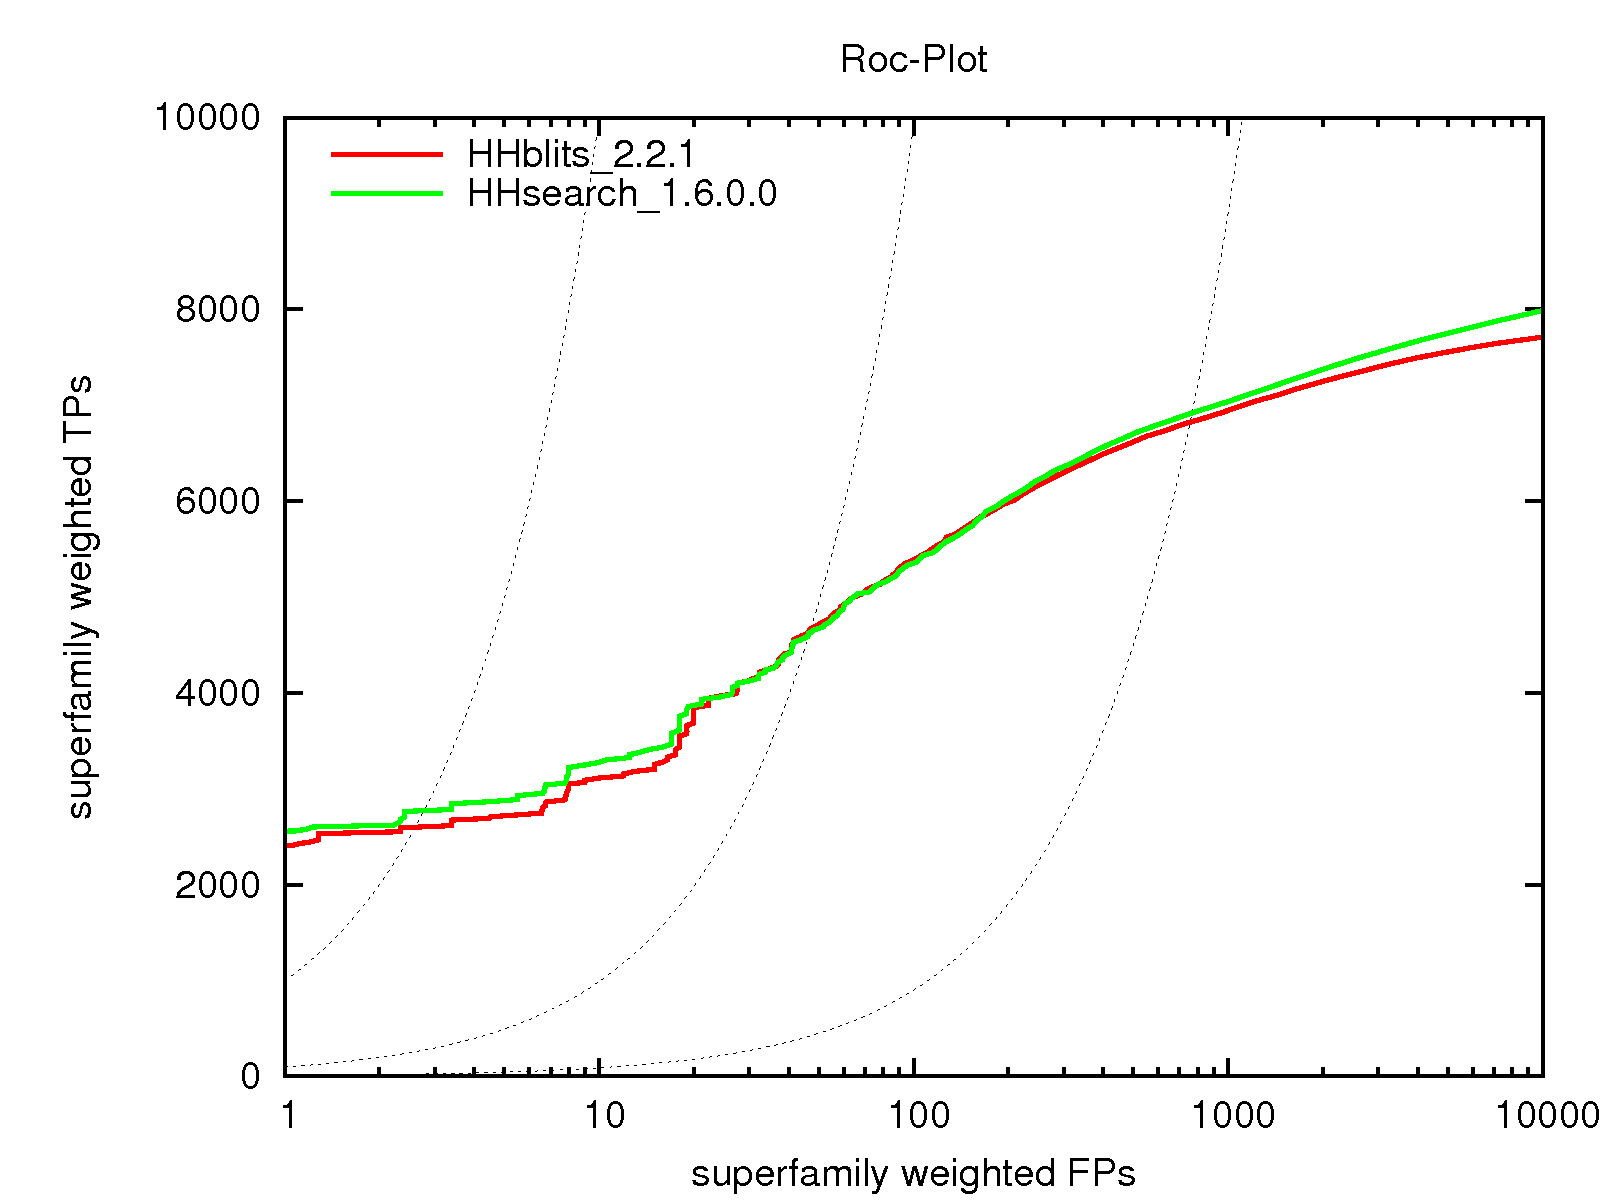
\includegraphics[width=0.5 \textwidth]{hhblits-hhsearch.png}
\caption{Benchmark of HHsearch and HHblits on a SCOP20 dataset.}
\label{fig:hhsearch_hhblits_bench}
\end{center}
\end{figure}

The HHblits tool can be used in much the same way as HHsearch. 
It takes the same input data and produces a results file in the same format as HHsearch.
Most of the HHsearch options also work for HHblits, which has
additional options associated with its extended functionality for iterative searches. 
Due to its fast prefilter, HHblits runs between 30 and 3000 times faster than HHsearch
at the cost of only a few percent lower sensitivity (Fig. \ref{fig:hhsearch_hhblits_bench}).

The same search as above is performed here using HHblits instead of HHsearch:
\begin{verbatim}
$ hhblits  -cpu 4 -i data/query.a3m -d dbs/scop70_1.75 -o data/query.hhr -n 1
\end{verbatim}

HHblits first scans the column state sequences in \verb`scop70_1.75_cs219.ffdata` with its fast prefilter. HMMs whose column state sequences pass the prefilter are read from the packed file \verb`scop70_1.75_hhm.ffdata` (using the index file \verb`scop70_1.75_hhm.ffindex`) and are aligned to the query HMM generated from \verb`query.a3m` using the slow Viterbi HMM-HMM alignment algorithm. The search results are written to the default output file \verb`query.hhr`. The option \verb`-n 1` tells HHblits to perform a single search iteration. (The default is 2 iterations.)


\subsection{Generating a multiple sequence alignment using HHblits}\label{msa_hhblits}

To generate an MSA for a sequence or initial MSA in query.a3m, the database to be searched should cover the entire sequence space, such as uniprot20 or nr20. The option \verb`-oa3m <msa_file>` tells HHblits to generate an output MSA from the significant hits, \verb`-n 1` specifies a single search iteration.
\begin{verbatim}
$ hhblits -cpu 4 -i data/query.seq -d dbs/uniprot20 -oa3m query.a3m -n 1
\end{verbatim}

At the end of the search, HHblits reads from the packed database file containing the MSAs the sequences belonging to HMMs with E-value below the threshold. The E-value threshold for inclusion into the MSA can be specified using the \verb`-e <E-value>` option. After the search, \verb`query.a3m` will contain the MSA in A3M format.

We could do a second search iteration, starting with the MSA from the previous search, to add more sequences. Since the MSA generated after the previous search contains more information than the single sequence in \verb`query.seq`, searching with this MSA will probably result in many more homologous database matches.
\begin{verbatim}
$ hhblits -cpu 4 -i query.a3m -d dbs/uniprot20 -oa3m query.a3m -n 1
\end{verbatim}
Instead, we could directly perform two search iterations starting from \verb`query.seq`:
\begin{verbatim}
$ hhblits -cpu 4 -i data/query.seq -d dbs/uniprot20 -oa3m query.a3m -n 2 
\end{verbatim}
See section \ref{2_vs_1+1} for an explanation why the results can be slightly different.

In practice, it is recommended to use between 1 and 4 iterations for building MSAs, depending on the trade-off between reliability and specificity on one side and sensitivity for remotely homologous sequences on the other side. The more search iterations are done, the higher will be the risk of non-homologous sequences or sequence segments entering the MSA and recruiting more of their kind in subsequent iterations. This is particularly problematic when searching with sequences containing short repeats, regions with amino acid compositional bias and, although less dramatic,  with multiple domains. Fortunately, this problem is much less pronounced in hhblits as compared to PSI-BLAST due to hhblits's lower number of iterations, its more robust Maximum Accuracy alignment algorithm, and the higher precision of its HMM-HMM alignments. 

The parameter \verb`mact` (maximum accuracy threshold) lets you choose the trade-off between sensitivity and 
precision. With a low mact-value (e.g.\ \verb`-mact 0.01`) very sensitive, but not 
so precise alignments are generated, whereas a search with a high mact-value (e.g.\ \verb`-mact 0.9`) 
results in shorter but very precise alignments. The default value of mact in HHblits is $0.35$ 
(changed from 0.5 in the beta version). 

To avoid unnecessarily large and diverse MSAs, HHblits stops iterating when the diversity of the query MSA -- measured as number of effective sequences, see section \ref{aliformats} -- grows passed a threshold of 10.0. This threshold can be modified with the \verb`--neffmax <float>` option. See subsection \ref{hhmformat} for a description of how the number of effective sequences is calculated in HHsuite.

To avoid the final MSAs to grow unnecessarily large, by default the database MSAs that are going to be merged with the query MSA into the result MSA are filtered with the active filter options (by default \verb`-id 90` and \verb`-diff 1000`). The \verb`-all` option turns off the filtering of the result MSA. Use this option if you want to get all sequences in the significantly similar uniprot20 clusters: 
\begin{verbatim}
$ hhblits -cpu 4 -i data/query.seq -d dbs/uniprot20 -oa3m query.a3m -all
\end{verbatim}

The A3M format uses small letters to mark inserts and capital letters to designate match and delete columns (see subsection \ref{aliformats}), allowing you to omit gaps aligned to insert columns. The A3M format therefore uses much less space for large alignments than FASTA but looks misaligned to the human eye. Use the \verb`reformat.pl` script to reformat \verb`query.a3m` to other formats, e.g.\ for reformatting the MSA to Clustal and FASTA format, type
\begin{verbatim}
$ reformat.pl a3m clu query.a3m query.clu
$ reformat.pl a3m fas query.a3m query.fas
\end{verbatim}

Next, to add secondary structure information to the MSA we call the script \verb`addss.pl`. For \verb`addss.pl` to work, you have to make sure that the paths to BLAST and PSIPRED in the file \verb`$HHLIB/scripts/HHPaths.pm` are correctly filled in. Then type
\begin{verbatim}
$ addss.pl query.a3m
\end{verbatim}
When the sequence has a SCOP or PDB identifier as first word in its name, the script tries to add the DSSP states as well. Open the \verb`query.a3m` file and check out the two lines that have been added to the MSA. Now you can generate a hidden Markov model (HMM) from this MSA:
\begin{verbatim}
$ hhmake -i query.a3m
\end{verbatim}
The default output file is \verb`query.hhm`. By default, the option \verb`-M first` will 
be used. This means that exactly those columns of 
the MSAs which contain a residue in the query sequence will be assigned to Match 
/ Delete states, the others will be assigned to Insert states. (The query sequence is 
the first sequence not containing secondary structure information.) Alternatively, you 
may want to apply the 50\%-gap rule by typing \verb`-M 50`, which assigns only those columns 
to Insert states which contain more than 50\% gaps. The \verb`-M first` option makes sense 
if your alignment can best be viewed as a seed sequence plus aligned homologs to 
reinforce it with evolutionary information. This is the case in the SCOP and PDB 
versions of our HMM databases, since here MSAs are built around a single seed 
sequence (the one with known structure). On the contrary, when your alignment 
represents an entire family of homologs and no sequence in particular, it is best to 
use the 50\% gap rule. This is the case for Pfam or SMART MSAs, for instance. 
Despite its simplicity, the 50\% gap rule has been shown to perform well in practice.

When calling \verb`hhmake`, you may also apply several filters, such as maximum pairwise 
sequence identity (\verb`-id <int>`), minimum sequence identity with query sequence 
(\verb`-qid <int>`), or minimum coverage with query (\verb`-cov <int>`). But beware 
of reducing the diversity of your MSAs too much, as this will lower the sensitivity to
detect remote homologs.

Previous versions of HHsuite (the 'HHsearch package') included a perl script \verb`buildali.pl` to build MSAs for a query sequence using PSI-BLAST as its search engine. Because HHblits performs better than PSI-BLAST in all aspects that we have tested, we decided to remove this script from HHsuite. It can still be downloaded as part of HHsearch version 1.5.0.


\subsection{Visually checking an MSA for corrupted regions}

Iterative search methods such as PSI-BLAST and HHblits may generate alignments containing non-homologous sequence stretches or even large fractions of non-homologous sequences. The cause for this is almost always the overextension of homologous alignments into non-homologous regions. This has been termed \emph{homologous overextension} in \cite{Gonzalez:2010}. This effect occurs particularly in multidomain and repeat proteins. A single overextended alignment in the search results leads to more of such sequences to be included in the profile of the next iteration -- usually all homologous to the first problematic sequence but with even longer non-homologous stretches. Thus, after three or more iterations, large sections of the resulting MSA may be non-homologous to the original query sequence. This risk of homologous overextension is greatly reduced in HHblits in comparison to PSI-BLAST, because fewer iterations are usually necessary for HHblits and because HHblits uses the Maximum Accuracy alignment algorithm (see section \ref{MAC}), which is much less prone to overextend alignments than the Smith-Waterman/Viterbi algorithm used by most other programs including PSI-BLAST. Still, in important cases it is worth to visually check the MSAs of the query and the matched database protein for the presence of corrupted regions containing non-homologous sequence stretches. 

The recommended procedure to visually check an MSA is the following. We first reduce the MSA to a small set of sequences that could still fit into a single window of an alignment viewer:
\begin{verbatim}
$ hhfilter -i query.a3m -o query.fil.a3m -diff 30
\end{verbatim}
The option \verb`-diff` causes hhfilter to select a representative set of at least 30 sequences that best represent the full diversity of the MSA. Sequences that contain non-homologous stretches are therefore usually retained, as they tend to be the most dissimilar to the main sequence cluster. 

Next, we remove all inserts (option \verb`-r`) with respect to the first, master sequence in the MSA. The resulting MSA is sometimes called a master-slave alignment:
\begin{verbatim}
$ reformat.pl -r query.fil.a3m query.fil.fas
\end{verbatim}

This alignment is now very easy to inspect for problematic regions in any viewer that allows to color the residues according to their physico-chemical properties. We can recommend \verb`alnedit` (downloadable from \url{www.eb.tuebingen.mpg.de/?id=421}) or \verb`jalview`, for example:
\begin{verbatim}
$ java -jar ~/bioinfo/alnedit.jar query.fil.fas .
\end{verbatim}
%Here is an example of a corrupted MSA, visualized as described here with alnedit
%\begin{figure}[h]
%\begin{center}
%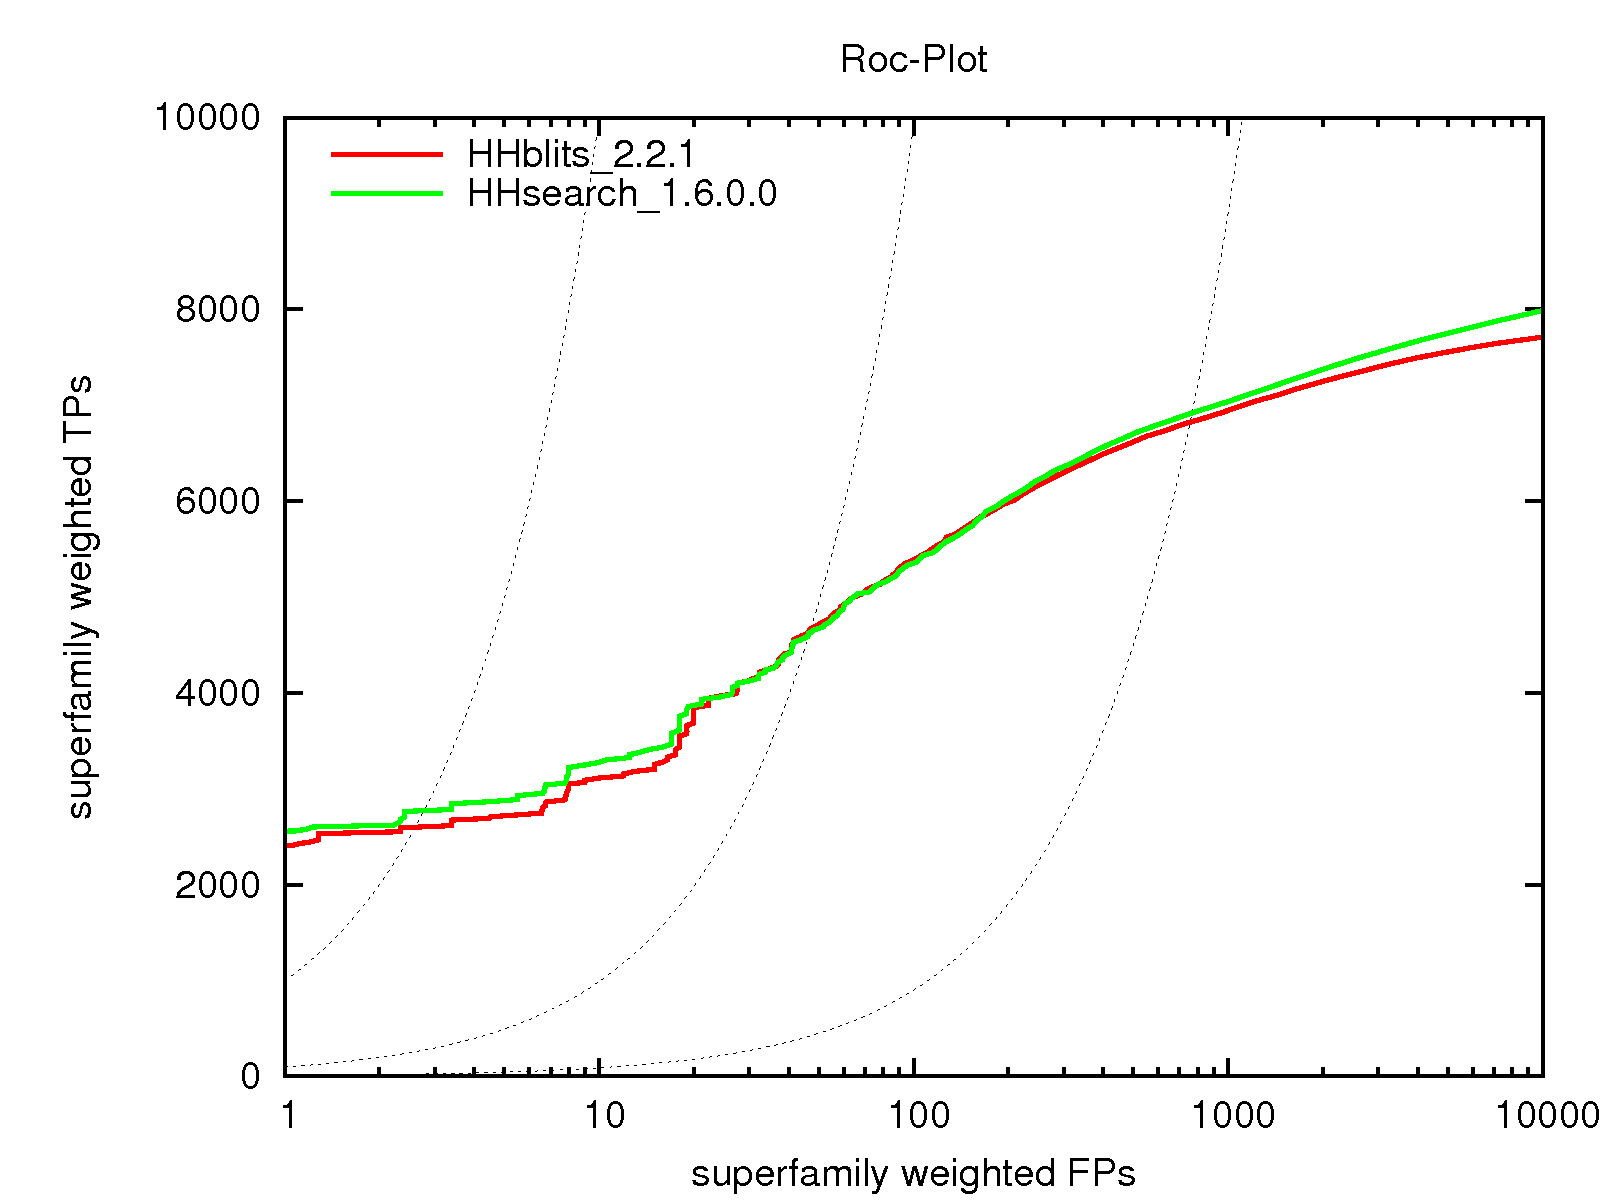
\includegraphics[width=0.5 \textwidth]{hhblits-hhsearch.png}
%\caption{Corrupted alignment: The master-slave MSA for sequence XXXX generated using three iterations of PSI-BLAST shows ...}
%\label{fig:hhsearch_hhblits_bench}
%\end{center}
%\end{figure}





\subsection{Building customized databases} \label{building_dbs}

It is simple to build custom HHsuite databases using the same tools we use to build the standard HHsuite databases (except uniprot20). An example application is to search for homologs among all proteins of an organism. To build your own HHsuite database from a set of sequences, you first need to generate an MSA with predicted secondary structure for every sequence in the set.

First of all we split the concatenated fasta file to an ffindex with ffindex\_from\_fasta.

\begin{verbatim}
$ ffindex_from_fasta -s <db>_fas.ff{data,index} <db.fas> 
\end{verbatim}

Now, to build an MSA with HHblits for each sequence in \verb`<db>_fas.ff{data,index}`, run\\[-1mm]

\begin{verbatim}
$ mpirun -np <number_threads> ffindex_apply_mpi <db>_fas.ff{data,index} \\
    -i <db>_a3m_wo_ss.ffindex -d <db>_a3m_wo_ss.ffdata -- 
    hhblits -d <path_to/uniprot20> -i stdin -oa3m stdout -n 2 -cpu 1
\end{verbatim}

The MSAs are written to the ffindex \verb`<db>_a3m_wo_ss.ff{data,index}`. To be sure that everything went smoothly, check that the number of lines in \verb`<db>_a3m.ffindex` is the same as the number of lines in \verb`<db>_fas.ffindex`. 

The number of HHblits search iterations and the HMM inclusion E-value threshold for HHblits can be changed from their default values (2 and 0.01, respectively) using the \verb`'-n <int>'` and \verb`'-e <float>'` options. A higher number of iterations such as  \verb`'-n 3'` will result in very high sensitivity to discover remotely homologous relationships, but the ranking among homologous proteins will often not reflect their degree of relationship to the query. The reason is that any similarities that are higher than the similarities among the sequences in the query and database MSAs cannot be resolved. 

Now, add PSIPRED-predicted secondary structure and if possible DSSP secondary structure annotation to all MSAs:
\begin{verbatim}
$ mpirun -np <number_threads> ffindex_apply_mpi <db>_a3m_wo_ss.ff{data,index} \\
    -i <db>_a3m.ffindex -d <db>_a3m.ffdata -- addss.pl stdin stdout 
$ rm <db>_wo_ss_a3m.ff{data,index}
\end{verbatim}

We also need to generate an HHM file for each MSA file:

\begin{verbatim}
$ mpirun -np <number_threads> ffindex_apply_mpi <db>_a3m.ff{data,index} \\
    -i <db>_hhm.ffindex -d <db>_hhm.ffindex -- hhmake -i stdin -o stdout -v 0
\end{verbatim}

In order to build the ffindex containing the column state sequences for prefiltering for each a3m we run:

\begin{verbatim}
$ OMP_NUM_THREADS=<number_threads> cstranslate -A ${HHLIB}/data/cs219.lib \\
    -D ${HHLIB}/data/context_data.lib -x 0.3 -c 4 -f -i <db>_a3m \\
    -o <db>_cs219 -I a3m -b
$ ffindex_build -as <db>_cs219.ff{data,index}
\end{verbatim}

Next we want to optimize the hmm and a3m ffindices. For this purpose we sort the files in the
data files according to the number of columns in the MSAs. The number of columns can be retrieved
in the third row of \verb`<db>_cs219.ffindex`.

\begin{verbatim}
$ sort -k3 -n <db>_cs219.ffindex | cut -f1 > sorting.dat

$ ffindex_order sorting.dat <db>_hhm.ff{data,index} <db>_hhm_ordered.ff{data,index}
$ mv <db>_hhm_ordered.ffindex <db>_hhm.ffindex
$ mv <db>_hhm_ordered.ffdata <db>_hhm.ffdata

$ ffindex_order sorting.dat <db>_a3m.ff{data,index} <db>_a3m_ordered.ff{data,index}
$ mv <db>_a3m_ordered.ffindex <db>_a3m.ffindex
$ mv <db>_a3m_ordered.ffdata <db>_a3m.ffdata
\end{verbatim}

As with all perl/python scripts and binaries in the HHsuite, a list of additional options can be retrieved by calling the scripts without parameters.


\subsection{Modifying or extending existing databases}

Assume you have a list of filenames in \verb`files.dat` you want to remove from an HHsuite database.

\begin{verbatim}
$ ffindex_modify -s -u -f files.dat <db>_a3m.ffindex
$ ffindex_modify -s -u -f files.dat <db>_hhm.ffindex
$ ffindex_modify -s -u -f files.dat <db>_cs219.ffindex
\end{verbatim}

This deletes the file entries from the ffindex files, however the files are still in the ffdata file.
This way HHblits and HHsuite won't be able to use them. If you want to get rid of them in the ffdata file
you may re-optimize the databases.

\begin{verbatim}
$ ffindex_build -as <db>_cs219_ordered.ff{data,index} \\
    -i <db>_cs219.ffindex -d <db>_cs219.ffdata
$ mv <db>_c219_ordered.ffindex <db>_cs219.ffindex
$ mv <db>_cs219_ordered.ffdata <db>_cs219.ffdata

$ sort -k3 -n <db>_cs219.ffindex | cut -f1 > sorting.dat

$ ffindex_order sorting.dat <db>_hhm.ff{data,index} <db>_hhm_ordered.ff{data,index}
$ mv <db>_hhm_ordered.ffindex <db>_hhm.ffindex
$ mv <db>_hhm_ordered.ffdata <db>_hhm.ffdata

$ ffindex_order sorting.dat <db>_a3m.ff{data,index} <db>_a3m_ordered.ff{data,index}
$ mv <db>_a3m_ordered.ffindex <db>_a3m.ffindex
$ mv <db>_a3m_ordered.ffdata <db>_a3m.ffdata
\end{verbatim}

If you want to check your HHsuite database you may run:
\begin{verbatim}
$ hhsuitedb.py -o <db> --cpu 1
\end{verbatim}

\verb`hhsuitedb.py` supports the flag \verb`--force` that tries to fix the database.
This may lead to the deletion of MSAs from the database.

Additionally you may add a3m, hhm and cs219 files with globular expressions to an existing database.
Please keep in mind that related a3m, hhm and cs219 files should have the same name. To make it easier
you may add just a3m files and the corresponding hhm and cs219 files will be calculated by the script.
\begin{verbatim}
$ hhsuitedb.py -o <db> --cpu 1 --ia3m=<a3m_glob> --ics219=<cs219_glob> --ihhm=<hhm_glob>
\end{verbatim}

\section{Frequently asked questions}

\subsection{How do I report a bug? \label{report-bug}}
If you think you found a bug, PLEASE report it to us. But we would be grateful if you could first make sure that the problem is not due to wrong usage or wrong file formats. Please reread the relevant sections of the user guide and check for possible warnings. Rerun the command with verbose option \verb`-v 3` or \verb`-v 4` to see if you can find where things go awry. If the problem persists, we will need everything to reproduce the bug on our machines. Please send us (1) the input file, (2) the database name and version, or, if it is not a standard database, the link to your ftp server to download the database files, (3) the output files, best with -v 3 or -v 4 option, (4) the command and its screen output, (5) the operating system and CPU description on which the bug occurred. Under Linux, please send the output of 
\small
\begin{verbatim}
$ echo $HHLIB $PATH; uname -a; lsb_release -a; head -n 25 /proc/cpuinfo; ulimit -a; free
\end{verbatim}
\normalsize
to \url{soeding@mpibpc.mpg.de}. Thanks a lot!

\subsection{What is HMM-HMM comparison and why is it so powerful?}
When searching for remote homologs, it is wise to make use of as much information about the query and database proteins as possible in order to better distinguish true from false positives and to produce optimal alignments. This is the reason why sequence-sequence comparison is inferior to profile-sequence comparison. Sequence profiles contain for each column of a multiple alignment the frequencies of the 20 amino acids. They therefore contain detailed information about the conservation of each residue position, i.e., how important each position is for defining other members of the protein family, and about the preferred amino acids. Profile Hidden Markov Models (HMMs) are similar to simple sequence profiles, but in addition to the amino acid frequencies in the columns of a multiple sequence alignment they contain information about the frequency of inserts and deletions at each column. Using profile HMMs in place of simple sequence profiles should therefore further improve sensitivity. Using HMMs both on the query and the database side greatly enhances the sensitivity/selectivity and alignment quality over sequence-profile based methods such as PSI-BLAST. HHsearch is the first software to employ HMM-HMM comparison and HHblits is the first profile-profile comparison method that is fast enough to do iterative searches to build MSAs. 

\subsection{When can the HHsuite be useful for me?}
Sequence search methods such as BLAST, FASTA, or PSI-BLAST are of prime importance for biological research because functional information of a protein or gene can be inferred from homologous proteins or genes identified in a sequence search. But quite often no significant relationship to a protein of known function can be established. This is certainly the case for the most interesting group of proteins, those for which no ortholog has yet been studied. In cases where conventional sequence search methods fail, HHblits and HHsearch quite often allow to make inferences from more remotely homologous relationships. HHblits builds better MSAs, with which more remote homologs can then be found using HHsearch or HHblits, e.g.\ by searching the PDB or domain databases such as Pfam. If the relationship is so remote that no common function can be assumed, one can often still derive hypotheses about possible mechanisms, active site positions and residues, or the class of substrate bound \cite{Todd:2001, Pawlowski:2000}. When a homologous protein with known structure can be identified, its stucture can be used as a template to model the 3D structure of the protein of interest \cite{Rychlewski:1998}, since even protein domains that shared a common ancestor some 3 billion years ago mostly have similar 3D structures \cite{Kinch:2002,Soding:2006a,Alva:2010}. The 3D model may then help to generate hypotheses to guide experiments. 

\subsection{What does homology mean and why is it important?}
Two protein sequences are homologous to each other if they descended from a common ancestor sequence. Generally, homologous proteins (or protein fragments) have similar structure because structures diverge much more slowly than their sequences \cite{Chothia:1986}. Depending on the degree of divergence between the sequences, the proteins may also have similar cellular functions, ligands, protein interaction partners, or enzymatic mechanisms \cite{Todd:2001}. On the contrary, proteins that have a similar structure by convergence (i.e., by chance) are said to be analogous. They don't generally share similar functions or biochemical mechanisms and are therefore much less helpful for making inferences. HHsearch and HHblits are tools for homology detection and as such do not normally detect analogous relationships \cite{Alva:2010,Remmert:2010}.


\subsection{How can I verify if a database match is homologous?}
Here is a list of things to check if a database match really is at least locally homologous.
 
{\bf Check probability and E-value}:
HHsearch and HHblits can detect homologous relationships far beyond the twilight zone, i.e., below 20\% sequence identity. Sequence identity is therefore not an appropriate measure of relatedness anymore. The estimated probability of the template to be (at least partly) homologous to your query sequence is the most important criterion to decide whether a template HMM is actually homologous or just a high-scoring chance hit. When it is larger than 95\%, say, the homology is nearly certain. Roughly speaking, one should give a hit serious consideration (i.e., check the other points in this list) whenever (1) the hit has $>50\%$ probability, or (2) it has $>30\%$ probability and is among the top three hits. The E-value is an alternative measure of statistical significance. It tells you how many chance hits with a score better than this would be expected if the database contained only hits unrelated to the query. At E-values below one, matches start to get marginally significant. Contrary to the probability, when calculating the E-value HHsearch and HHblits do not take into account the secondary structure similarity. Therefore, the probability is a more sensitive measure than the E-value.

{\bf Check if homology is biologically suggestive or at least reasonable}:
Does the database hit have a function you would expect also for your query? Does it come from an organism that is likely to contain a homolog of your query protein?

{\bf Check secondary structure similarity}:
If the secondary structure of query and template is very different or you can't see how they could fit together in 3D, then this is a reason to distrust the hit. Note however that if the query alignment contains only a single sequence, the secondary structure prediction is quite unreliable and confidence values are overestimated.

{\bf Check relationship among top hits}: 
If several of the top hits are homologous to each other, (e.g.\ when they are members of the same SCOP superfamily), then this will considerably reduce the chances of all of them being chance hits, especially if these related hits are themselves not very similar to each other. Searching the SCOP database is very useful precisely for this reason, since the SCOP family identifier (e.g.\ a.118.8.2) allows to tell immediately if two templates are likely homologs.

{\bf Check for possible conserved motifs}:
Most homologous pairs of alignments will have at least one (semi-)conserved motif in common. You can identify such putative (semi-)conserved motifs by the agglomeration of three or more well-matching columns (marked with a '\verb`|`' sign between the aligned HMMs) occurring within a few residues, as well as by matching consensus sequences. Some false positive hits have decent scores due to a similar amino acid composition of the template. In these cases, the alignments tend to be long and to lack conserved motifs.

{\bf Check residues and role of conserved motifs}: 
If you can identify possible conserved motifs, are the corresponding conserved template residues involved in binding or enzymatic function?

{\bf Check query and template alignments}: 
A corrupted query or template alignment is the main source of high-scoring false positives. The two most common sources of corruption in an alignment are (1) non-homologous sequences, especially repetitive or low-complexity sequences in the alignment, and (2) non-homologous fragments at the ends of the aligned database sequences. Check the query and template MSAs in an alignment viewer such as Jalview or ALNEDIT.

{\bf Realign with other parameters}: 
change the alignment parameters. Choose global instead of local mode, for instance, if you expect your query to be globally homologous to the putative homolog. Try to improve the probability by changing the values for minimum coverage or minimum sequence identity. You can also run the query HMM against other databases.

{\bf Build the query and/or database MSAs more aggressively}:
If your query (or template) MSA is not diverse enough, you could increase sensitivity substantially by trying to include more remotely homologous sequences into the MSA. Try using our HHsenser web server at \url{http://toolkit.tuebingen.mpg.de/hhsenser} \cite{Soding:2006b}. Check the HHsenser alignment manually using an alignment editor. Have non-homologous sequences or sequence segments been accidentally included? You can also try to build a more diverse MSA manually: Inspect the HHblits results after the first iteration and consider including hits above the E-value inclusion threshold of 0.001, based on biological plausibility, relatedness of the organism, a reasonable looking alignment, or just guessing. Then start the second HHblits search iteration HHblits with this manually enriched alignment. 

{\bf Try out other tools}:
Try other tools (e.g.\ for profile-profil comparison) and servers for remote homology detection and structure prediction. 
A list of servers can be found in \cite{Mariani:2011} and \cite{Battey:2007}.

{\bf Verify predictions experimentally}: 
The ultimate confirmation of a homologous relationship or structural model is, of course, the experimental verification of some of its key predictions, such as validating the binding to certain ligands by binding assays, measuring biochemical activity, or comparing the knock-out phenotype with the one obtained when the putative functional residues are mutated.


\subsection{What does the maximum accuracy alignment algorithm do?} \label{MAC}
HHblits and HHsearch use a better alignment algorithm than the quick and 
standard Viterbi method to generate the final HMM-HMM alignments. Both realign
all displayed alignments in a second stage using the more accurate Maximum Accuracy 
(MAC) algorithm \cite{Durbin:2008,Biegert:2008}. The Viterbi algorithm is employed 
for searching and ranking the matches. The realignment step is parallelized 
(\verb`-cpu <int>`) and typically takes a few seconds only.    

Please note: Using different alignment algorithms for scoring and aligning has the 
disadvantage that the pairwise alignments that are displayed are not always very similar to 
those that are used to calculate the scores. This can lead to confusing results 
where alignments of only one or a few residues length may have obtained significant
E-values. In such cases, run the search again with the \verb`-norealign` option, which will 
skip the MAC-realignment step. This will allow you to check if the Viterbi alignments 
are valid at all, which they will probably not be. The length of the MAC alignments 
can therefore give you additional information to decide if a match is valid. In order
to avoid confusion for users of our HHpred server \cite{Soding:2005b, Hildebrand:2009}, 
the \verb`-norealign` option is the default there, whereas for you pros who dare to use 
the command line package, realigning is done by default.

The posterior probability threshold is controlled with the \verb`-mact` option. 
This parameter controls the alignment algorithm's greediness. More precisely, the 
MAC algorithm finds the alignment that maximizes the sum of posterior probabilities 
minus mact for each aligned pair. Global alignments are generated with -mact 0, 
whereas -mact 0.5 will produce quite conservative local alignments. 

The -global and -local options now refer to both the Viterbi search stage as 
well as the MAC realignment stage. With -global (-local), the posterior probability 
matrix will be calculated for global (local) alignment. When -global is used in 
conjunction with -realign, the mact parameter is automatically set to 0 in order to 
produce global alignments. In other words, both following two commands will give 
global alignments:
\begin{verbatim}
$ hhsearch -i <query> -d <db> -realign -mact 0
$ hhsearch -i <query> -d <db> -realign -global
\end{verbatim}

The first version uses \emph{local} Viterbi to search and then uses MAC to realign the 
proteins globally (since mact is 0) on a \emph{local} posterior probability matrix. The 
second version uses \emph{global} Viterbi to search and then realigns globally (since mact 
is automatically set to 0) on a \emph{global} posterior matrix. To detect and align remote 
homologs, for which sometimes only parts of the sequence are conserved, the first 
version is clearly better. It is also more robust. If you expect to find globally 
alignable sequence homologs, the second option might be preferable. In that case, 
it is recommended to run both versions and compare the results. 

\subsection{How is the MSA diversity Neff calculated?} \label{Neff}
The number of effective sequences of the full alignment, which appears as NEFF in the header of each hhm file, is the average of local values \verb`Neff_M(i)` over all alignment positions $i$. The values \verb`Neff_M(i)` are given in the main model section of the hhm model files (subsection \ref{hhmformat}). They quantify the \emph{local} diversity of the alignment in a region around position $i$. More precisely, \verb`Neff_M(i)` measures the diversity of subalignment $Ali_M(i)$ that contains all sequences that have a residue at column $i$ of the full alignment. The subalignment contains all columns for which at least 90\% of these sequences have no end gap. End gaps are gaps to the left of the first residue or to the right of the last residue. The latter condition ensures that the sequences in the subalignment $Ali_M(i)$ cover most of the columns in it. The number of effective sequences in the subalignment $Ali_M(i)$ is exp of the average sequence entropy over all columns of the subalignment. Hence, \verb`Neff_M` is bounded by 0 from below and 20 from above. In practice, it is bounded by the entropy of a column with background amino acid distribution $f_a$: $N_\mathrm{eff} < \sum_{a=1}^{20} f_a \log f_a \approx 16$. Similarly, \verb`Neff_I(i)` gives the diversity of the subalignment $Ali_I(i)$ of all sequences that have an insert at position $i$, and \verb`Neff_D(i)` refers to the diversity of subaligment $Ali_D(i)$ of all sequences that have a Delete (a gap) at position $i$ of the full alignment. 



\subsection{On how to use HHsuite tools}

{\bf Do HHsearch and HHblits work fine with multi-domain sequences?}
HHblits and HHsearch have been designed to work with multi-domain queries. However, the chances for false positives entering the query alginment during the HHblits iterations is greater for multi-domain proteins. For long sequences, it may therefore be of advantage to first search the PDB or the SCOP domain database and then to cut the query sequence into smaller parts on the basis of the identified structural domains. Pfam or CDD are - in our opinion - less suitable to determine domain boundaries.

{\bf How do I best build HMMs for integral membrane proteins?}
Despite the biased amino acid composition in their integral membrane helices, membrane proteins behave very well in HMM-HMM comparisons. In many benchmark tests and evolutionary studies we have not noticed any higher rates of false positives than with cytosolic proteins. 

{\bf How do I reconcile overlapping and conflicting domain predictions}, for example when domain A is predicted from residues 2-50 with 98\% probability and domain B from 2-200 with 95\% probability? The probability that a pair of residues is correctly aligned is the product of the probability for the database match to be homologous (given by the values in the \verb`Probab` column of the hit list) times the posterior probability of the residue pair to be correctly aligned given the database match is correct in the first place. The posterior probabilities are specified by the confidence numbers in the last line of the alignment blocks (0 corresponds approximately to 0-10\%, 9 to 90-100\%). Therefore, an obvious solution would be to prune the alignments in the overlapping region such that the sum of total probabilities is maximized. There is no script yet that does this automatically.

{\bf How can I build a phylogenetic tree for HMMs?}
I would use a similarity measure like the raw score per alignment length. You might also add the secondary structure score to the raw score with some weight. Whereas probabilities, E-values, and P-values are useful for deciding whether a match is a reliable homolog or not, they are not suitable for measuring similarities because they strongly depend on the length of the alignment, roughly like $\mathrm{P-value} \propto \exp(\lambda \times \mathrm{average\_similarity} \times \mathrm{length})$, with some constant $\lambda$ of order 1. The probability has an even more complex dependence on length. Also, the ``Similarity'' given above the alignment blocks is a simple substitution matrix score per column between the query and template master sequences and does not capture the evolutionary information contained in the MSAs (see subsection \ref{aliblocksformat}). One note of caution: Large, diverse MSAs are usually more sensitive to find homologs than narrower ones. Therefore, I would limit the diversity of all HMMs to some reasonable number (perhaps around 5 or 7, depending on how far diverged your HMMs are). This filtering can be done using \verb`$ hhfilter -i <MSA.a3m> -o <MSA_filt.a3m> -neff 5`. 

{\bf Can I weight some residues more than others during the HMM-HMM alignment?} For example to select templates for homology modeling, it could make sense to weight residues around the known functional site more strongly. This might also positively impact the query-template alignment itself. Well, directly weighting query or template match states is not possible. What you can do with a bit of file fiddling, however, may even be better: You can modify the amount of pseudocounts that hhblits, hhsearch, or hhalign will automatically add to the various match state columns in the query or template profile HMM. This is equivalent to assuming a higher conservation for these positions, since pseudocounts are basically mutations that are added to the observed counts in the training sequences to generalize to more remotely related sequences. In HHsuite, the more diverse the sequence neighborhood around a match state column $i$ is, as measured by the number of effective sequences \verb`Neff_M(i)` (see subsection \ref{Neff}), the fewer pseudocounts are added. By manually increasing \verb`Neff_M(i)` for a match state column you increase the assumed conservation of this position in the protein. The \verb`Neff_M(i)` values are found in the hhm-formatted HMM model files in the eighth column of the second line of each match state block in units of $0.001$ (see subsection \ref{hhmformat}). You could, for example, simply increase \verb`Neff_M(i)` values by a factor of two for important, conserved positions. Setting \verb`Neff_M(i)` to 99999 will reduce pseudocounts to effectively zero. A word of caution is advised: HMMs built from a diverse set of training sequences already contain quantitative information about the degree of conservation for each position.


{\bf Don't I need to calibrate my query or database HMMs anymore?}
No. If you don't specify otherwise, the two parameters of the extreme-value distribution for the query are estimated by a neural network from the lengths and diversities ($N_\mathrm{eff}$)) of query and database HMMs that was trained on a large set of example queries-template pairs, in an approach similar to the one used in \cite{Sadreyev:2008}. However, the old calibration is still available as an option in HHsearch.

{\bf Should I use the \verb`-global` option to build MSAs} for an HHsuite database if I am intersted in global alignments to these database HMMs?
Never use \verb`-global` when building MSAs by iterative searches with HHblits. Remember that global alignments are very greedy alignments, where alignments stretch to the ends of either query of database HMM, no matter what. Global alignments will therefore often lead to non-homologous segments getting included in the MSA, which is catastrophic, as these false segments will lead to many false positive matches when searching with this MSA. But you may use \verb`-global` when searching (with a single iteration) for global matches of your query HMMs through your customized HHsuite database, for example.

{\bf How many iterations of hhblits should I use to search my customized genome database?} One iteration! Doing more than one search iterations in general only makes sense in order to build up a diverse MSA of homologous sequences by searching through the uniprot20 or nr20 databases. 



\subsection{About HHsuite databases}


{\bf How can I retrieve database A3M or HHM files from my HHsuite database?}
For reasons of efficiency, the MSA A3M and HHM model files are packed into two files, \verb`<db>_a3m.ffdata` and \verb`<db>_hhm.ffdata`, each with its own index file. The contained files are easy to extract from the packed files. For example, to dump \verb`d1aa7a_.a3m` in \verb`scop70` to standard output, type 
\begin{verbatim}
$ ffindex_get scop70_a3m.ffdata scop70_a3m.ffindex d1aa7a_.a3m
\end{verbatim}
You may write the extracted file to a separate file by appending \verb`'> d1aa7a_.a3m'` to the above command.
If you want to extract all files in the ffindex data structures to directory \verb`tmp/scop70`, type
\begin{verbatim}
$ ffindex_unpack scop70_a3m.ffdata scop70_a3m.ffindex tmp/scop70/ .
\end{verbatim}

{\bf How can I build my own UniProt database for HHblits?}
The procedure to cluster the nr or UniProt databases is more complicated than building a database for a genome or for the sequences in the pdb. As its first step it involves clustering these huge databases down to 20\%-30\% sequence identity. The clustering is done in our lab using a new method, kClust (Hauser M, Mayer CE, and S\"oding J., to be published), available under GPL at \url{ftp://ftp://toolkit.lmb.uni-muenchen.de/kClust/}. We will add all scripts to build these HHsuite databases to the HHsuite in due time. These scripts generate A3M files, HHM files, and consensus sequences. Because of the large number of files to generate, these scripts need to be run on a computer cluster and this would require considerable computer savvyness. 

{\bf Will you offer an HHsuite database that includes environmental sequences?}
We have not seen significant improvements in remote homology detection through inclusion of environmental sequences. A problem with these sequences is their low quality, in particular chimeric sequences from wrong assemblies. This can lead to corrupted profiles in iterative searches. We therefore have no immediate plans to provide a UniProt+env or nr+env for hhblits. If you think you really need the env sequences, you have to use our old \verb`buildali.pl` script or PSI-BLAST for the time being. An alternative is to use kClust to cluster the database yourself. See the previous question.

{\bf How do I read the sequence/HMM headers in the pdb70 databases?}
The pdb70 database is clustered to 70\% maximum pairwise sequence identity to reduce redundancy. The PDB identifiers at the end of the description line of sequence $X$ lists the sequences with lower experimental resolution that were removed for having higher than 70\% sequence identity with PDB sequence $X$. The asterisks indicate that a multi-atom ligand is bound in the structure. 


\subsection{About unexpected HHsuite behavior and troubleshooting}

{\bf Why do I get different results when reversing the roles of query and template?} When taking A as the query, the pairwise alignment and significance scores with template B in the database can be different than when B is the query and A the template. By default hhblits, hhsearch, and hhalign add context-specific pseudocounts to the query MSA or HMM whereas the much faster substitution matrix pseudocounts are added to the database HMMs/MSAs for reasons of speed. If you want to combine the significance estimates from the forward and reverse comparisons, we recommend to take the geometric mean of Probability, P-value and E-value. Since the less diverse HMM or MSA will profit more from the context-specific pseudocounts than the more diverse HMM or MSA, it might be even better to take the estimate from the comparison in which the HMM/MSA with the smaller diversity (measured as number of effective sequences, NEFF) is used as the query. 

{\bf Why do I sometimes get the same database hit twice with different probabilities?} Each line in the summary hit list refers to an alignment with an HMM in the database, not to the database HMM itself. Sometimes, alternative (suboptimal) alignments covering a different part of either the query or the database HMM may appear in the hit list. Usually, both the optimal and the alternative alignments are correct, in particular when the query or the database HMMs represent repeat proteins. 

{\bf Why do I get different results using hhblits and hhsearch} when I search with the same query through the same database? There are two reasons. First, some hits that hhsearch shows might not have passed the prefilter in hhblits. The option \verb`-prepre_smax_thresh <bits>` lets you modify the minimum score threshold of the first, gapless alignment prefilter (default is 10 bits). Option \verb`-pre_evalue_thresh <E-value>` sets the maximum E-value threshold for the second, gapped alignment prefilter (default is 1000). Second, while the probabilities and P-values of hhblits and hhsearch should be the identical for the same matches, the E-values are only similar. The reason is that hhblits heuristically combines the E-values of the second prefilter with the E-values from the full HMM-HMM Viterbi alignment into total E-values \cite{Remmert:2011}. These E-values are slightly better in distinguishing true from false hits, because they combine the partly independent information from two comparisons.

{\label{2_vs_1+1} \bf Why do I get different results when I perform $2$ and $1+1$ iterations with HHblits?} When you do a single iteration and start a second iteration with the A3M output file from the first iteration, the alignments should be nearly the same as if you do two iterations (\verb`-n 2`) Why not exactly the same? Because when doing multiple iterations in a single hhblits run, alignments for each hit are only calculated once. When the same database HMM is found in later search iterations, the ``frozen'', first alignment is used instead of recomputing it. This increases robustness with respect to homologous overextension. However, the significance values can be slightly different between the cases with$2$ and $1+1$ iterations. The reason is that the HHblits P-value is calculated by a weighted combination of the P-value of the Viterbi pairwise HMM alignment and the prefilter E-value. The prefilter E-values differ in the two cases described, since in the first case the E-value is calculated for the first prefilter search (before the first full search) and in the second case it is calculated for the second prefilter search, performed with the query MSA obtained \emph{after} the first search iteration. 

{\bf Why do I get a segmentation fault when calling hhblits on our new machine?}
Often, segmentation faults can be caused by too little available memory. HHblits needs memory to read the entire column state file into memory for prefiltering (\verb`*.cs219`). For Viterbi HMM-HMM alignment it needs about 
\begin{equation}
\textrm{Memory Viterbi} = \textrm{Query\_length} \times \textrm{max\_db\_seq\_length} \times (\textrm{num\_threads}+1) \times 5 \textrm{B} \,. 
\end{equation}
Here, num\_threads is the number of threads specified with option \verb`-cpu <int>`. For realignment, HHblits needs in addition 
\begin{equation}
\textrm{Memory Realing} = \textrm{Query\_length} \times \textrm{max\_db\_seq\_length} \times (\textrm{num\_threads}+1) \times 8 \textrm{B} \,, 
\end{equation}
but the amount of memory for realignment can be limited using the \verb`-maxmem <GB>` option, which will cause the realignment to skip the longest sequences. Under Linux, you can check your memory limit settings using \verb`ulimit -a`. Make sure you have at least 4GB per thread. Try 
\begin{verbatim}
$ ulimit -m 4000000 -v 4000000 -s 8192 -f 4000000
\end{verbatim}
Also try using \verb`-cpu 1 -maxmem 1` to reduce memory requirements. If it still does not work, follow the tipps in subsection \ref{report-bug} to report your problems to us.



\section{HHsearch/HHblits output: hit list and pairwise alignments}\label{outformat}

\subsection{Summary hit list}

Let's do a search with the human PIP49/FAM69B protein, for which we generated an MSA in \verb`query.a3m` with two iterations of HHblits in subsection \ref{msa_hhblits}:

\scriptsize
\begin{verbatim}
Search results will be written to query.hhr
query.a3m is in A2M, A3M or FASTA format
Read query.a3m with 272 sequences
Alignment in query.a3m contains 431 match states
149 out of 270 sequences passed filter (up to 91% position-dependent max pairwise sequence identity)
Effective number of sequences exp(entropy) = 5.2 
.................................................. 1000 HMMs searched
.................................................. 2000 HMMs searched
.................................................. 3000 HMMs searched
.................................................. 4000 HMMs searched
.................................................. 5000 HMMs searched
.................................................. 6000 HMMs searched
.................................................. 7000 HMMs searched
.................................................. 8000 HMMs searched
.................................................. 9000 HMMs searched
.................................................. 10000 HMMs searched
.................................................. 11000 HMMs searched
.................................................. 12000 HMMs searched
.................................................. 13000 HMMs searched
....................................
Realigning 183 query-template alignments with maximum accuracy (MAC) algorithm ...

Query         sp|Q5VUD6|FA69B_HUMAN Protein FAM69B OS=Homo sapiens GN=FAM69B PE=2 SV=3
Match_columns 431
No_of_seqs    149 out of 272
Neff          5.2 
Searched_HMMs 13730
Date          Wed Jan  4 17:44:24 2012
Command       hhsearch -i query.a3m -d /cluster/user/soeding/databases/scop -cpu 18 

 No Hit                             Prob E-value P-value  Score    SS Cols Query HMM  Template HMM
  1 d1qpca_ d.144.1.7 (A:) Lymphoc  99.7 4.5E-17 3.2E-21  154.3  10.2   99  203-320    56-157 (272)
  2 d1jpaa_ d.144.1.7 (A:) ephb2 r  99.7 4.3E-17 3.1E-21  156.8   8.8   99  203-321    75-177 (299)
  3 d1uwha_ d.144.1.7 (A:) B-Raf k  99.7 5.1E-17 3.7E-21  154.8   7.7  100  203-322    52-154 (276)
  4 d1opja_ d.144.1.7 (A:) Abelson  99.7 6.2E-17 4.5E-21  154.8   8.3  100  203-321    61-164 (287)
  5 d1mp8a_ d.144.1.7 (A:) Focal a  99.6 9.9E-17 7.2E-21  151.3   8.6  100  203-322    56-158 (273)
  6 d1sm2a_ d.144.1.7 (A:) Tyrosin  99.6 1.2E-16 8.8E-21  150.3   8.8   99  203-321    48-150 (263)
  7 d1u59a_ d.144.1.7 (A:) Tyrosin  99.6 2.4E-16 1.7E-20  150.9   9.5   99  203-321    57-158 (285)
  8 d1xbba_ d.144.1.7 (A:) Tyrosin  99.6 2.2E-16 1.6E-20  150.2   8.6   97  203-320    56-155 (277)
  9 d1vjya_ d.144.1.7 (A:) Type I   99.6 2.6E-16 1.9E-20  151.3   8.8   98  204-320    46-156 (303)
 10 d1mqba_ d.144.1.7 (A:) epha2 r  99.6 4.4E-16 3.2E-20  148.0   8.7  193  203-422    57-272 (283)
...
 64 d1j7la_ d.144.1.6 (A:) Type II  97.3 0.00014   1E-08   65.0   6.3   33  292-324   184-216 (263)
 65 d1nd4a_ d.144.1.6 (A:) Aminogl  96.7  0.0012 8.5E-08   58.5   6.6   31  292-322   176-206 (255)
 66 d1nw1a_ d.144.1.8 (A:) Choline  96.6  0.0011 7.8E-08   63.9   5.8   37  203-239    92-128 (395)
 67 d2pula1 d.144.1.6 (A:5-396) Me  95.6  0.0071 5.2E-07   58.3   6.4   32  290-322   222-253 (392)
 68 d1a4pa_ a.39.1.2 (A:) Calcycli  91.7    0.12 8.9E-06   40.0   5.4   62  140-202    18-80  (92)
 69 d1ksoa_ a.39.1.2 (A:) Calcycli  91.2    0.17 1.2E-05   39.5   5.8   56  147-203    28-83  (93)
 70 d1e8aa_ a.39.1.2 (A:) Calcycli  90.5    0.23 1.7E-05   38.3   6.0   56  147-203    27-82  (87)
...
175 d1qxpa2 a.39.1.8 (A:515-702) C  23.7      29  0.0021   28.8   3.8   49  137-197    69-118 (188)
176 d1tuza_ a.39.1.7 (A:) Diacylgl  23.5      55   0.004   25.3   5.3   55  143-201    44-106 (118)
177 d1ggwa_ a.39.1.5 (A:) Cdc4p {F  23.1      26  0.0019   27.0   3.2   66  129-197    35-101 (140)
178 d1topa_ a.39.1.5 (A:) Troponin  22.8      72  0.0052   24.5   6.0   58  140-199    65-123 (162)
179 d1otfa_ d.80.1.1 (A:) 4-oxaloc  22.5      66  0.0048   21.5   5.0   40  267-306    12-53  (59)
180 d1oqpa_ a.39.1.5 (A:) Caltract  22.2      32  0.0023   24.0   3.2   32  165-197     3-34  (77)
181 d1df0a1 a.39.1.8 (A:515-700) C  21.7      43  0.0032   27.0   4.5   51  137-199    67-118 (186)
182 d1zfsa1 a.39.1.2 (A:1-93) Calc  21.1      41   0.003   24.6   3.8   30  170-199     8-38  (93)
183 d1snla_ a.39.1.7 (A:) Nucleobi  20.9      23  0.0016   26.2   2.2   24  174-197    18-41  (99)

Done
\end{verbatim}
\normalsize
 
The summary hit list that is written to the screen shows the best hits from the 
database, ordered by the probability of being a true positive (column 4: 'Prob'). 
The meaning of the columns is the following:
\vspace{5mm}

\renewcommand{\arraystretch}{1.2}

\begin{description}
\item{\verb`No`}: the index of the datbase match.

\item{\verb`Hit`}: the first 30 characters of the name line.

\item{\verb`Prob`}: the Probability of template to be a true positive.
For the probability of being a true positive, the secondary structure score 
in column \verb`SS` is taken into account, together with the raw score in\
column \verb`Score`. 
True positives are defined to be either globally homologous or they are at least 
homologous in parts, and thereby locally similar in structure. More precisely, 
the latter criterion demands that the MAXSUB score between query and hit is at 
least 0.1. In almost all cases the structural similarity will we be due to a global
OR LOCAL homology between query and template.

\item{\verb`E-value`}:
The E-value gives the average number of false positives ('wrong hits') with a score 
better than the one for the template when scanning the database. It is a measure of 
reliability: E-values near to 0 signify a very reliable hit, an E-value of 10 means 
about 10 wrong hits are expected to be found in the database with a score at least 
this good. Note that E-value and P-value are calculated without taking the secondary 
structure into account!


\item{\verb`P-value`}: 
The P-value is the E-value divided by the number of sequences in the database.
It is the probability that in a \emph{pairwise} comparison a wrong hit will score at least 
this good.

\item{\verb`Score`}: the raw score is computed by the Viterbi HMM-HMM alignment excluding the
secondary structure score. It is the sum of similarities of the aligned profile columns
minus the position-specific gap penalties in bits. The column similarity score is the 
log-sum-of-odds score (base 2) as described in the original HHsearch paper 
(Soding, Bioinformatics 2005). The gap penalties are the log2 of the state transition
probabilities, e.g. from match state to insert or delete to match state.

\item{\verb`SS`}: the secondary structure score.
This score tells you how well the PSIPRED-predicted (3-state) or actual DSSP-determined 
(8-state) secondary structure sequences agree with each other. PSIPRED confidence 
values are used in the scoring, low confidences getting less statistical weight.

\item{\verb`Cols`}: the number of aligned Match columns in the HMM-HMM alignment.

\item{\verb`Query HMM`}: the range of aligned match states from the query HMM.

\item{\verb`Template HMM`}: the range of aligned match states from the database/template HMM and, 
in parenthesis, the number of match states in the database HMM.

\end{description}



\subsection{HMM-HMM pairwise alignments}\label{aliblocksformat}

The output file d1bpya1.hhr contains the same hit list plus the pairwise HMM alignments. One example is give here:

\scriptsize
\begin{verbatim}
No 68 
>d1a4pa_ a.39.1.2 (A:) Calcyclin (S100) {Human (Homo sapiens), P11 s100a10, calpactin [TaxId: 9606]}
Probab=91.65  E-value=0.12  Score=40.00  Aligned_cols=62  Identities=16%  Similarity=0.149  Sum_probs=42.0

Q ss_pred             ccCCCCCCcHHHHHHHHHHHHHhhcccCccHHHHHHHHHhhhhccCCCCcCHHHHHHH-HHHHH
Q sp|Q5VUD6|FA69  140 FDKPTRGTSIKEFREMTLSFLKANLGDLPSLPALVGQVLLMADFNKDNRVSLAEAKSV-WALLQ  202 (431)
Q Consensus       140 ~d~p~~g~s~~eF~emv~~~i~~~lg~~~~l~~L~~~~~~~~d~nk~g~vs~~e~~sl-waLlq  202 (431)
                      ||+..-..|.+||.+++.......++.+.+ ...+..++..+|.|+||+|++.|...+ ..|..
T Consensus        18 yd~ddG~is~~El~~~l~~~~~~~~~~~~~-~~~v~~~~~~~D~n~DG~I~F~EF~~li~~l~~   80 (92)
T d1a4pa_          18 FAGDKGYLTKEDLRVLMEKEFPGFLENQKD-PLAVDKIMKDLDQCRDGKVGFQSFFSLIAGLTI   80 (92)
T ss_dssp             HHGGGCSBCHHHHHHHHHHHCHHHHHHSCC-TTHHHHHHHHHCTTSSSCBCHHHHHHHHHHHHH
T ss_pred             HcCCCCEEcHHHHHHHHHHhccccccccCC-HHHHHHHHHHHhCCCCCCCcHHHHHHHHHHHHH
Confidence            444433449999999998876655554332 234566677899999999999997544 44443
\end{verbatim}\normalsize

This alignment shows an EF hand embedded in a kinase domain in PIP49/FAM69B. The first line, 
which begins with with a ``\verb`>`'', contains the name and description line of the template/database 
HMM. (We use ``template HMM'' and ``matched database HMM'' synonymously.) 
The next line summarizes the main statistics for the alignment: The probability for the query and 
template HMMs to be homologous (\verb`Probab`), the \verb`E-value`, the raw \verb`Score`, and the 
number of aligned columns are repeated from the summary hit list. The \verb`Identities` give the percentage
of aligned residue pairs of the query and the template master sequences that are identical. 
The \verb`Similarity` is the arithmetic mean of the substitution scores between the aligned residue
pairs from the query and template master sequences. The substitution matrix is the same as the
one used to calculate the pseudocounts for the database HMMs, by default the Gonnet matrix. 
(The matrix can be changed with the \verb`-Blosom<XX>` option.) 

The \verb`Sum_probs` value is the sum over the posterior probabilities of all aligned pairs 
of match states. These probabilities are calculated by the Forward-Backward algorithm. 
(They are used by the maximum accuracy algorithm 
which computes the final alignments.) When the template HMM has secondary structure annotation from
DSSP, the \verb`sum_probs` value runs only over aligned pairs for which the template has a 
valid DSSP state, not a \verb`-` sign. A  \verb`-` would indicate that the structural coordinates of
that residue are missing in the template. For homology modelling, this special treatment of templates 
with known structure makes \verb`sum_probs` a useful feature to use for ranking templates.



The pairwise alignment consists of one or more blocks with the following lines:

\small
\begin{verbatim}
Q ss_dssp:      the query secondary structure as determined by DSSP (when available)
Q ss_pred:      the query secondary structure as predicted by PSIPRED (when available)
Q <Q_name>:     the query master sequence
Q Consensus:    the query alignment consensus sequence
\end{verbatim}\normalsize

The predicted secondary structure states are shown in capital letters if the PSIPRED
confidence value is between 0.7 and 1.0, for lower confidence values they are given 
in lower-case letters. With the option {\tt '-ssconf'}, {\tt 'ss\_conf'} lines can 
be added to the alignments which report the PSIPRED confidence values by numbers 
between 0 and 9 (as in versions up to 1.5).

The consensus sequence uses capital letters for well conserved columns and
lower case for partially conserved columns. Unconserved columns are marked by 
a tilde \verb`~`. Roughly speaking, amino acids that occur with $\ge 60\%$ probability 
(before adding pseudocounts) are written as capital letters and amino acids that have 
$\ge 40\%$ probability are written as lower case letters, where gaps are included
in the fraction counts. More precisely, when the gap-corrected amino acid fraction
    \[p_i(a)*N_\mathrm{eff}(i)/(N_\mathrm{eff}+1)\]
is above 0.6 (0.4) an upper (lower) case letter is used for amino acid a.
Here, $p_i(a)$ is the emission probability for a in column i, $N_\mathrm{eff}$ is the effective 
number of sequences in the entire multiple alignment (between 1 and 20) and $N_\mathrm{eff}(i)$ is 
the effective number of sequences in the subalignment consisting of those sequences
that do not have a gap in column i. These percentages increase
approximately inversely proportionally with the fraction of gaps in the column, 
hence a column with only cysteines and 50\% gaps gets a lower case letter.
              
The line in the middle shows the column score between the query and template 
amino acid distributions. It gives a valuable indication for the alignment quality.
\small
\begin{verbatim}
  = : column score below -1.5
  - : column score between -1.5 and -0.5
  . : column score between -0.5 and +0.5
  + : column score between +0.5 and +1.5
  | : column score above   +1.5
\end{verbatim}\normalsize

A unit of column score corresponds approximately to 0.6 bits.
From the column score line the excellent alignment around the conserved 
{\tt 'D.n.DG.i...E'} motif in the turn between two helices is evident. The alignment around the 
gap by contrast scores only a bit better than zero per residue and is
therefore not very reliable.

After the template block, which consists of the following lines, 
\small 
\begin{verbatim}
T Consensus:    the template alignment consensus sequence
T <T_name>:     the template domain sequence
T ss_dssp:      the template secondary structure as determined by DSSP (when available)
T ss_pred:      the template secondary structure as predicted by PSIPRED (when available)
\end{verbatim}\normalsize

The last line in the block ({\tt Confidence}) reports the reliability of the pairwise 
query-template alignment. The confidence values are obtained from the posterior 
probabilities calculated in the Forward-Backward algorithm. A value of 8 indicates
a probability that this pair of HMM columns is correctly aligned between 0.8 and 0.9. 
The {\tt Confidence} line is only displayed when the -realign option is active.


\section{File formats}

\subsection{Multiple sequence alignment formats} \label{aliformats}

Multiple alignments can be read in A2M, A3M, or aligned FASTA format. (Check the -M option for 
using an input format different from the default A3M). You can transform MSAs 
from Clustal or Stockholm format to A3M or aligned FASTA with the \verb`reformat.pl` utility 
supplied in this package. 

To reformat from Clustal format to A3M:
\begin{verbatim}
  $ reformat.pl test.aln test.a3m
\end{verbatim}
or explicitly, if the formats can not be recognized from the extensions:
\begin{verbatim}
  $ reformat.pl clu a3m test.clustal test.a3m
\end{verbatim}
To reformat from Stockholm to aligned FASTA:
\begin{verbatim}
  $ reformat.pl test.sto test.fas
\end{verbatim}


\subsubsection*{Example for aligned FASTA format:}

\scriptsize
\begin{verbatim}
>d1a1x__ b.63.1.1 (-) p13-MTCP1 {Human (Homo sapiens)}
PPDHLWVHQEGIYRDEYQRTWVAVVEE--E--T--SF---------LR----------ARVQQIQVPLG-------DAARPSHLLTS-----QL
>gi|6678257|ref|NP_033363.1|:(7-103) T-cell lymphoma breakpoint 1 [Mus musculus]
HPNRLWIWEKHVYLDEFRRSWLPVVIK--S--N--EK---------FQ----------VILRQEDVTLG-------EAMSPSQLVPY-----EL
>gi|7305557|ref|NP_038800.1|:(8-103) T-cell leukemia/lymphoma 1B, 3 [Mus musculus]
PPRFLVCTRDDIYEDENGRQWVVAKVE--T--S--RSpygsrietcIT----------VHLQHMTTIPQ-------EPTPQQPINNN-----SL
>gi|11415028|ref|NP_068801.1|:(2-106) T-cell lymphoma-1; T-cell lymphoma-1A [Homo sapiens]
HPDRLWAWEKFVYLDEKQHAWLPLTIEikD--R--LQ---------LR----------VLLRREDVVLG-------RPMTPTQIGPS-----LL
>gi|7305561|ref|NP_038804.1|:(7-103) T-cell leukemia/lymphoma 1B, 5 [Mus musculus]
----------GIYEDEHHRVWIAVNVE--T--S--HS---------SHgnrietcvt-VHLQHMTTLPQ-------EPTPQQPINNN-----SL
>gi|7305553|ref|NP_038801.1|:(5-103) T-cell leukemia/lymphoma 1B, 1 [Mus musculus]
LPVYLVSVRLGIYEDEHHRVWIVANVE--TshS--SH---------GN----------RRRTHVTVHLW-------KLIPQQVIPFNplnydFL
>gi|27668591|ref|XP_234504.1|:(7-103) similar to Chain A, Crystal Structure Of Murine Tcl1
-PDRLWLWEKHVYLDEFRRSWLPIVIK--S--N--GK---------FQ----------VIMRQKDVILG-------DSMTPSQLVPY-----EL
>gi|27668589|ref|XP_234503.1|:(9-91) similar to T-cell leukemia/lymphoma 1B, 5;
-PHILTLRTHGIYEDEHHRLWVVLDLQ--A--ShlSF---------SN----------RLLIYLTVYLQqgvafplESTPPSPMNLN-----GL
>gi|7305559|ref|NP_038802.1|:(8-102) T-cell leukemia/lymphoma 1B, 4 [Mus musculus] 
PPCFLVCTRDDIYEDEHGRQWVAAKVE--T--S--SH---------SPycskietcvtVHLWQMTTLFQ-------EPSPDSLKTFN-----FL
>gi|7305555|ref|NP_038803.1|:(9-102) T-cell leukemia/lymphoma 1B, 2 [Mus musculus]
---------PGFYEDEHHRLWMVAKLE--T--C--SH---------SPycnkietcvtVHLWQMTRYPQ-------EPAPYNPMNYN-----FL
\end{verbatim}\normalsize

The sequence name and its description must be contained in a single name line beginning 
with the $>$ symbol and followed directly by the sequence name. The residue data is 
contained in one or more lines of arbitrary length following the name line. No empty 
lines should be used. In aligned FASTA the gaps are written with '-' and the n'th 
letter of each sequence (except newlines) is understood to build the n'th column of the 
multiple alignment. 


\subsubsection*{The same alignment in A2M format looks like this:}

\scriptsize
\begin{verbatim}
>d1a1x__ b.63.1.1 (-) p13-MTCP1 {Human (Homo sapiens)}
PPDHLWVHQEGIYRDEYQRTWVAVVEE..E..T..SF.........LR..........ARVQQIQVPLG.......DAARPSHLLTS.....QL
>gi|6678257|ref|NP_033363.1|:(7-103) T-cell lymphoma breakpoint 1 [Mus musculus]
HPNRLWIWEKHVYLDEFRRSWLPVVIK..S..N..EK.........FQ..........VILRQEDVTLG.......EAMSPSQLVPY.....EL
>gi|7305557|ref|NP_038800.1|:(8-103) T-cell leukemia/lymphoma 1B, 3 [Mus musculus]
PPRFLVCTRDDIYEDENGRQWVVAKVE..T..S..RSpygsrietcIT..........VHLQHMTTIPQ.......EPTPQQPINNN.....SL
>gi|11415028|ref|NP_068801.1|:(2-106) T-cell lymphoma-1; T-cell lymphoma-1A [Homo sapiens]
HPDRLWAWEKFVYLDEKQHAWLPLTIEikD..R..LQ.........LR..........VLLRREDVVLG.......RPMTPTQIGPS.....LL
>gi|7305561|ref|NP_038804.1|:(7-103) T-cell leukemia/lymphoma 1B, 5 [Mus musculus]
----------GIYEDEHHRVWIAVNVE..T..S..HS.........SHgnrietcvt.VHLQHMTTLPQ.......EPTPQQPINNN.....SL
>gi|7305553|ref|NP_038801.1|:(5-103) T-cell leukemia/lymphoma 1B, 1 [Mus musculus]
LPVYLVSVRLGIYEDEHHRVWIVANVE..TshS..SH.........GN..........RRRTHVTVHLW.......KLIPQQVIPFNplnydFL
>gi|27668591|ref|XP_234504.1|:(7-103) similar to Chain A, Crystal Structure Of Murine Tcl1
-PDRLWLWEKHVYLDEFRRSWLPIVIK..S..N..GK.........FQ..........VIMRQKDVILG.......DSMTPSQLVPY.....EL
>gi|27668589|ref|XP_234503.1|:(9-91) similar to T-cell leukemia/lymphoma 1B, 5;
-PHILTLRTHGIYEDEHHRLWVVLDLQ..A..ShlSF.........SN..........RLLIYLTVYLQqgvafplESTPPSPMNLN.....GL
>gi|7305559|ref|NP_038802.1|:(8-102) T-cell leukemia/lymphoma 1B, 4 [Mus musculus] 
PPCFLVCTRDDIYEDEHGRQWVAAKVE..T..S..SH.........SPycskietcvtVHLWQMTTLFQ.......EPSPDSLKTFN.....FL
>gi|7305555|ref|NP_038803.1|:(9-102) T-cell leukemia/lymphoma 1B, 2 [Mus musculus]
---------PGFYEDEHHRLWMVAKLE..T..C..SH.........SPycnkietcvtVHLWQMTRYPQ.......EPAPYNPMNYN.....FL
\end{verbatim}\normalsize

A2M format is derived from aligned FASTA format. It looks very similar, but it 
distinguishes between match/delete columns and insert columns. This information is 
important to uniquely specify how an alignment is transformed into an HMM. The 
match/delete columns use upper case letters for residues and the '-' symbol for 
deletions (gaps). The insert columns use lower case letters for the inserted residues. 
Gaps aligned to inserted residues are written as '.' Lines beginning with a hash \# 
symbol will be treated as commentary lines in HHsearch/HHblits (see below).


\subsubsection*{The same alignment in A3M:}

\scriptsize
\begin{verbatim}
>d1a1x__ b.63.1.1 (-) p13-MTCP1 {Human (Homo sapiens)}
PPDHLWVHQEGIYRDEYQRTWVAVVEEETSFLRARVQQIQVPLGDAARPSHLLTSQL
>gi|6678257|ref|NP_033363.1|:(7-103) T-cell lymphoma breakpoint 1 [Mus musculus]
HPNRLWIWEKHVYLDEFRRSWLPVVIKSNEKFQVILRQEDVTLGEAMSPSQLVPYEL
>gi|7305557|ref|NP_038800.1|:(8-103) T-cell leukemia/lymphoma 1B, 3 [Mus musculus]
PPRFLVCTRDDIYEDENGRQWVVAKVETSRSpygsrietcITVHLQHMTTIPQEPTPQQPINNNSL
>gi|11415028|ref|NP_068801.1|:(2-106) T-cell lymphoma-1; T-cell lymphoma-1A [Homo sapiens]
HPDRLWAWEKFVYLDEKQHAWLPLTIEikDRLQLRVLLRREDVVLGRPMTPTQIGPSLL
>gi|7305561|ref|NP_038804.1|:(7-103) T-cell leukemia/lymphoma 1B, 5 [Mus musculus]
----------GIYEDEHHRVWIAVNVETSHSSHgnrietcvtVHLQHMTTLPQEPTPQQPINNNSL
>gi|7305553|ref|NP_038801.1|:(5-103) T-cell leukemia/lymphoma 1B, 1 [Mus musculus]
LPVYLVSVRLGIYEDEHHRVWIVANVETshSSHGNRRRTHVTVHLWKLIPQQVIPFNplnydFL
>gi|27668591|ref|XP_234504.1|:(7-103) similar to Chain A, Crystal Structure Of Murine Tcl1
-PDRLWLWEKHVYLDEFRRSWLPIVIKSNGKFQVIMRQKDVILGDSMTPSQLVPYEL
>gi|27668589|ref|XP_234503.1|:(9-91) similar to T-cell leukemia/lymphoma 1B, 5;
-PHILTLRTHGIYEDEHHRLWVVLDLQAShlSFSNRLLIYLTVYLQqgvafplESTPPSPMNLNGL
>gi|7305559|ref|NP_038802.1|:(8-102) T-cell leukemia/lymphoma 1B, 4 [Mus musculus] 
PPCFLVCTRDDIYEDEHGRQWVAAKVETSSHSPycskietcvtVHLWQMTTLFQEPSPDSLKTFNFL
>gi|7305555|ref|NP_038803.1|:(9-102) T-cell leukemia/lymphoma 1B, 2 [Mus musculus]
---------PGFYEDEHHRLWMVAKLETCSHSPycnkietcvtVHLWQMTRYPQEPAPYNPMNYNFL
\end{verbatim}\normalsize

The A3M format is a condensed version of A2M format. It is obtained by omitting all '.' 
symbols from A2M format. Hence residues emitted by Match states of the HMM are in upper 
case, residues emitted by Insert states are in lower case and deletions are written '-'.
A3M-formatted alignments can be reformatted to other formats like FASTA or A2M with 
the \verb`reformat.pl` utility:
\begin{verbatim}
  reformat.pl test.a3m test.a2m
\end{verbatim}
Lines beginning with a hash \# symbol will be treated as commentary lines in HHsearch/HHblits
(see below). Please note that A3M, though very practical and space-efficient, 
is not a standard format, and the name A3M is our personal invention.

\subsubsection*{Secondary structure information in A3M/A2M or FASTA MSAs for HHsearch/HHblits}

The alignments read in by HHblits, HHsearch or HHmake can also contain secondary structure 
information. This information can be included in sequences with special names, 
like in this A3M file:

\scriptsize
\begin{verbatim}
>ss_dssp
CCSEEEEEETTEEEETTSCEEEEEEEECSSCEEEEEECCCCCCCSCCCHHHHTTCSSCSEEEEETTTEEEETTSC
>aa_dssp
PPDHLWVHQEGIYRDEYQRTWVAVVEEETSFLRARVQQIQVPLGDAARPSHLLTSQLPLMWQLYPEERYMDNNSR
>aa_pred 
PPDHLWVHQEGIYRDEYQRTWVAVVEEETSFLRARVQQIQVPLGDAARPSHLLTSQLPLMWQLYPEERYMDNNSR
>ss_pred 
CCCEEEEECCCEECCCCCEEEEEEEEECCCCCCEEEEEEECCCCCCCCCCCCCCCCCCCEEEECCCCCEECCCCC
>ss_conf 
987689961870104587078999970578640132153103788788777774424614787217702035631
>d1a1x__ b.63.1.1 (-) p13-MTCP1 {Human (Homo sapiens)}
PPDHLWVHQEGIYRDEYQRTWVAVVEEETSFLRARVQQIQVPLGDAARPSHLLTSQLPLMWQLYPEERYMDNNSR
>gi|6678257|ref|NP_033363.1|:(7-103) T-cell lymphoma breakpoint 1 [Mus musculus]
HPNRLWIWEKHVYLDEFRRSWLPVVIKSNEKFQVILRQEDVTLGEAMSPSQLVPYELPLMWQLYPKDRYRSCDSM
>gi|7305557|ref|NP_038800.1|:(8-103) T-cell leukemia/lymphoma 1B, 3 [Mus musculus]
PPRFLVCTRDDIYEDENGRQWVVAKVETSRSpygsrietcITVHLQHMTTIPQEPTPQQPINNNSLPTMWRLESMNTYTGTDGT
>gi|11415028|ref|NP_068801.1|:(2-106) T-cell lymphoma-1; T-cell lymphoma-1A [Homo sapiens]
HPDRLWAWEKFVYLDEKQHAWLPLTIEikDRLQLRVLLRREDVVLGRPMTPTQIGPSLLPIMWQLYPDGRYRSSDSS
\end{verbatim}\normalsize

The sequence with name \verb`>ss_dssp` contains the 8-state DSSP-determined secondary
structure. \verb`>aa_dssp` and \verb`>aa_pred` contain the same residues as the query 
sequence (\verb`>d1a1x__` in this case). They are optional and used merely to check whether the 
secondary structure states have correctly been assigned to the alignment. \verb`>ss_pred` 
contains the 3-state secondary structure predicted by PSIPRED, and \verb`>ss_conf`
 contains the corresponding confidence values. The query sequence is the first sequence that 
does not start with a special name. It is not marked explicitly.


\subsubsection*{Name lines in alignments}

If you would like to create HMMs from alignments with a specified name which differ 
from the name of the first sequence, you can do so by adding name lines to 
your FASTA, A2M, or A3M alignment:

\scriptsize
\begin{verbatim}
#PF02043 Bac_chlorC:  Bacteriochlorophyll C binding protein
>ss_pred
CCCCHHHHHHHHHHHHHHHHHHHHHHHHHHHHHHHHHHHHHHCCCCCCCCCCCCCCCCCCCCCCCCCCCCHHHHHHHCC
>ss_conf
9863234658887677777750019999999998878886403445886666775655576678777660667633039
>CSMA_CHLAU/1-79
ATRGWFSESSAQVAQIGDIMFQGHWQWVSNALQATAAAVDNINRNAYPGVSRSGSGEGAFSSSPSNGFRPKRIRSRFNR
>CSMA_CHLPH/2-51
NGGGVFTDILAASGRIFEVMVEGHWATVGYLFDSLGKGVSRINQNAYGNM-----------------------------
...
\end{verbatim}\normalsize

When creating an HMM from an A3M file with hhmake, the first word of the name line is 
used as the name and file name of the HMM (PF02043 in this case). The following is an 
optional description. The descriptions will appear in the hit list and alignment section 
of the search results. The name lines can be arbitrarily long and there can be any number of 
name/description lines included, marked by a '\#' as the first character in the line. 
Note that name lines are read by HHmake but are not a part of the standard definition
of the FASTA or A2M format.
 

\subsection{HHsearch/HHblits model format (hhm-format)} \label{hhmformat}

HMMs can be read by HHsearch/HHblits in HHsuite's own hhm format.
Performance is severely reduced when using HMMER-format, because HMMER adds more pseudocounts than HHsearch/HHblits
that we cannot remove anymore. \emph{We therefore strongly advise against using models from HMMER with HHsuite.} 
We recommend to get the original MSA files and generate hhm-formatted models using \verb`hhmake`, as described in 
subsection \ref{msa_hhblits}.

If you absolutely need to use HMMER format, you can convert it to hhm format with \verb`hhmake`:
\begin{verbatim}
  $ hhmake -i test.hmm -o test.hhm
\end{verbatim}
This works only for a single HMM per file, not for concatenated HMMs. You 
may add predicted secondary structure to the hmm file with \verb`addss.pl` as for hhm format.

HHsearch/HHblits uses a format HMM that is unchanged since HHsearch version 1.5. 
This is the example of an HHM model file produced by HHmake:

\scriptsize
\begin{verbatim}
HHsearch 1.5
NAME  d1mvfd_ b.129.1.1 (D:) MazE {Escherichia coli}
FAM   b.129.1.1
FILE  d1mvfd_
COM   hhmake1 -i d1mvfd_.a3m -o test.hhm 
DATE  Wed May 14 10:41:06 2011
LENG  44 match states, 44 columns in multiple alignment
FILT  32 out of 35 sequences passed filter (-id 90 -cov 0 -qid 0 -qsc -20.00 -diff 100)
NEFF  4.0 
SEQ
>ss_dssp
CBCEEETTEEEEECCHHHHHHTTCCTTCBEEEEEETTEEEEEEC
>ss_pred
CCCCCCCCCCCCCCHHHHHHHHCCCCCCEEEEEEECCEEEEEEC
>ss_conf
93233467666600578899808998986889874993798739
>Consensus
sxIxKWGNSxAvRlPaxlxxxlxlxxgdxixxxxxxxxivlxPv
>d1mvfd_ b.129.1.1 (D:) MazE {Escherichia coli}
SSVKRWGNSPAVRIPATLMQALNLNIDDEVKIDLVDGKLIIEPV
>gi|10176344|dbj|BAB07439.1|:(1-43) suppressor of ppGpp-regulated growth inhibitor [Bacillus halodurans]
TTIQKWGNSLAVRIPNHYAKHINVTQGSEIELSLgSDQTIILKP-
>gi|50120611|ref|YP_049778.1|:(3-43) suppressor of growth inhibitory protein ChpA [Erwinia carotovora]
-TVKKWGNSPAIRLSSSVMQAFDMTFNDSFDMEIRETEIALIP-
>gi|44064461|gb|EAG93225.1|:(2-42) unknown [environmental sequence]
-SVVKWGSYLAVRLPAELVLELGLKEGDEIDLVKDDGPVRVR--
>gi|31442758|gb|AAP55635.1|:(1-44) PemI-like protein [Pediococcus acidilactici]
TRLAKWGNSKAARIPSQIIKQLKLDDNQDMTITIENGSIVLTPI
>gi|44419085|gb|EAJ13619.1|:(3-43) unknown [environmental sequence]
SAIQKWGNSAAVRLPAVLLEQIDASVGSSLNADVRPDGVLLSP-
>gi|24376549|gb|AAN57947.1|:(3-44) putative cell growth regulatory protein [Streptococcus mutans UA159]
SAINKWGNSSAIRLPKQLVQELQLQTNDVLDYKVSGNKIILEKV
>gi|11344928|gb|AAG34554.1|:(1-44) MazE [Photobacterium profundum]
TQIRKIGNSLGSIIPATFIRQLELAEGAEIDVKTVDGKIVIEPI
>gi|45681193|ref|ZP_00192636.1|:(2-44) COG2336: Growth regulator [Mesorhizobium sp. BNC1]
-TIRKIGNSEGVILPKELLDRHNLKTGDALAIVEEGSDLVLKPV
#
NULL  3706 5728 4211 4064 4839 3729 4763 4308 4069  3323  5509 4640 4464 4937 4285 4423 3815 3783 6325 4665
HMM   A    C    D    E    F    G    H    I    K     L     M    N    P    Q    R    S    T    V    W    Y
      M->M M->I M->D I->M I->I D->M D->D Neff NeffI NeffD
      0    *    *    0    *    0    *    *    *     *
S 1   *    *    *    *    *    *    *    *    *     *     *    *    *    *    *    1012 988  *    *    *   1
      0    *    *    *    *    *    *    2817 0     0

S 2   2307 *    *    *    *    *    *    *    *     *     *    *    *    3178 3009 2179 1546 *    *    *   2
      0    *    *    *    *    *    *    3447 0     0

V 3   *    *    *    *    *    *    *    917  *     3009  *    *    *    *    *    *    *    1530 *    *   3
      0    *    *    *    *    *    *    3447 0     0
  .
  .
  .
V 44  *    *    *    *    *    *    *    1309 *     *     *    *    *    *    *    *    *    745  *    *   44
      0    *    *    0    *    *    *    2533 0     0

//
\end{verbatim}
\normalsize

The first line (\verb`HHsearch 1.5`) gives the format version, which corresponds to the HHsearch version for which this format was first introduced. Newer versions of HHsearch/HHblits may use previous format versions. The \verb`NAME` line gives the name of the HMM and an optional description. The first 30 characters of this field are used in the summary hit list of the search results in hhr format, the full name line is given above the query-template alignments of the search results. The \verb`FAM` line contains the family if the sequence is from SCOP of PFAM (used for calibration). \verb`COM` is the command that was used to generate the file. \verb`NEFF` is the diversity of the alignment, calculated as $\exp$ of the negative entropy averaged over all columns of the alignment. 

The \verb`SEQ` section contains a number of aligned, representative (pseudo) sequences in A3M format and is terminated with a line containing only a \verb`#`. The first sequence represents the DSSP secondary structure (if available, i.e., if contained in the A3M or FASTA alignment from which the HMM model was built), the second and third sequences contain the predicted secondary structure and the corresponding confidence values in the range 0--9 (if available). The fourth sequence is the consensus annotation sequence that is shown in the pairwise query-template alignments in the hhsearch output. The first \emph{real} sequence after the pseudo sequences is the \emph{seed} or \emph{master} sequence from which the alignment was built (\verb`>d1mvfd_`, in our example). If the alignment does not represent a single master sequence but an entire family, as in the case of PFAM alignments for example, the first real sequence may be a consensus sequence calculated for the entire alignment. This master sequence is shown in the pairwise query-template alignments in the hhsearch output. 

The next line specifies the null model frequencies, which are extracted from the selected substitution matrix used to add pseudocounts. Each of the positive integers is equal to 1000 times the negative logarithm of the amino acid frequency (which is between 0 and 1):
\begin{equation}
  -1000 \times \log_2( frequency)
  \label{transformation}
\end{equation}
 After the two annotation lines that specify the order of columns for the emission and transition probabilities that follow, there is a line which is not currently read by HHsearch and that lists the transition frequencies from the begin state to the first Match state, Insert state and Delete state.

 The last block contains two lines for each column of the HMM. The first line starts with the amino acid in the master sequence at that column in the HMM and the column number. Following are 20  positive integers representing the match state amino acid emission frequencies (see eq.\ \ref{transformation}). Asterisks \verb`*` stand for a frequency of 0 (which would otherwise be represented by 99999). Please note that, unlike in HMMER format,  \emph{the emission frequencies do not contain pseudo-counts} in the HHsearch model format. The second line contains the seven transition frequencies (eq.\ \ref{transformation}) coded as in eq.\ \ref{transformation}. The three local diversities, \verb`Neff_M`, \verb`Neff_I`, and \verb`Neff_D` are given in units of 0.001 (see next paragraph). The end of the model is indicated by a line containing only \verb`//`.


\section{Summary of command-line parameters}

This is just a brief summary of command line parameters for the various binaries and
perl scripts as they are displayed by the programs when calling them without 
command line parameters. On the help pages of the HHpred/HHblits web server
\url{http://toolkit.tuebingen.mpg.de} you can find more detailed explanations
about some of the input parameters  ('Parameters' section) and about how to interpret
the output ('Results' section). The FAQ section contains valuable practical hints on topics
such as how to validate marginally significant database matches or how to avoid high-scoring
false positives.


\subsection{{\tt hhblits} -- HMM-HMM-based lighting-fast iterative sequence search}

HHblits is a sensitive, general-purpose, iterative sequence search tool that represents
both query and database sequences by HMMs. You can search HHsuite databases starting
with a single query sequence, a multiple sequence alignment (MSA), or an HMM. HHblits
prints out a ranked list of database HMMs/MSAs and can also generate an MSA by merging
the significant database HMMs/MSAs onto the query MSA.

The binary hhblits\_omp supports the parallelization over several queries with OpenMP.
In this case the input needs to be the basename of an ffindex with MSA's.
The outputs are treated as the basenames for output ffindices.

Assume the ffindex database \verb`/home/user/databases/scop_a3m.ff{data,index}`, the corresponding basename
is \verb`/home/user/databases/scop_a3m`

\small 
\begin{verbatim}
Usage: hhblits -i query [options] 
 -i <file>      input/query: single sequence or multiple sequence alignment (MSA)
                in a3m, a2m, or FASTA format, or HMM in hhm format

<file> may be 'stdin' or 'stdout' throughout.

Options:                                                                        
 -d <name>      database name (e.g. uniprot20_29Feb2012)                        
                Multiple databases may be specified with '-d <db1> -d <db2> ...'
 -n     [1,8]   number of iterations (default=2)                               
 -e     [0,1]   E-value cutoff for inclusion in result alignment (def=0.001)       

Input alignment format:                                                       
 -M a2m         use A2M/A3M (default): upper case = Match; lower case = Insert;
               ' -' = Delete; '.' = gaps aligned to inserts (may be omitted)   
 -M first       use FASTA: columns with residue in 1st sequence are match states
 -M [0,100]     use FASTA: columns with fewer than X% gaps are match states   
 -tags/-notags  do NOT / do neutralize His-, C-myc-, FLAG-tags, and trypsin 
                recognition sequence to background distribution (def=-notags)  

Output options: 
 -o <file>      write results in standard format to file (default=<infile.hhr>)
 -oa3m <file>   write result MSA with significant matches in a3m format
 -opsi <file>   write result MSA of significant matches in PSI-BLAST format
 -ohhm <file>   write HHM file for result MSA of significant matches
 -oalis <name>  write MSAs in A3M format after each iteration
 -add_cons      generate consensus sequence as master sequence of query MSA (default=don't)
 -hide_cons     don't show consensus sequence in alignments (default=show)     
 -hide_pred     don't show predicted 2ndary structure in alignments (default=show)
 -hide_dssp     don't show DSSP 2ndary structure in alignments (default=show)  
 -show_ssconf   show confidences for predicted 2ndary structure in alignments
 -Ofas <file>   write pairwise alignments in FASTA xor A2M (-Oa2m) xor A3M (-Oa3m) format   
 -seq <int>     max. number of query/template sequences displayed (default=1)  
 -aliw <int>    number of columns per line in alignment list (default=80)       
 -p [0,100]     minimum probability in summary and alignment list (default=20)  
 -E [0,inf[     maximum E-value in summary and alignment list (default=1E+06)      
 -Z <int>       maximum number of lines in summary hit list (default=500)        
 -z <int>       minimum number of lines in summary hit list (default=10)        
 -B <int>       maximum number of alignments in alignment list (default=500)     
 -b <int>       minimum number of alignments in alignment list (default=10)     

Prefilter options                                                               
 -noprefilt                disable all filter steps                                        
 -noaddfilter              disable all filter steps (except for fast prefiltering)         
 -maxfilt                  max number of hits allowed to pass 2nd prefilter (default=20000)   
 -min_prefilter_hits       min number of hits to pass prefilter (default=100)               
 -prepre_smax_thresh       min score threshold of ungapped prefilter (default=10)               
 -pre_evalue_thresh        max E-value threshold of Smith-Waterman prefilter score (default=0)
 -pre_bitfactor            prefilter scores are in units of 1 bit / pre_bitfactor (default=4)
 -pre_gap_open             gap open penalty in prefilter Smith-Waterman alignment (default=20)
 -pre_gap_extend           gap extend penalty in prefilter Smith-Waterman alignment (default=4)
 -pre_score_offset         offset on sequence profile scores in prefilter S-W alignment (default=50)

Filter options applied to query MSA, database MSAs, and result MSA              
 -all           show all sequences in result MSA; do not filter result MSA      
 -id   [0,100]  maximum pairwise sequence identity (def=90)
 -diff [0,inf[  filter MSAs by selecting most diverse set of sequences, keeping 
                at least this many seqs in each MSA block of length 50 
                Zero and non-numerical values turn off the filtering. (def=1000) 
 -cov  [0,100]  minimum coverage with master sequence (%) (def=0)             
 -qid  [0,100]  minimum sequence identity with master sequence (%) (def=0)    
 -qsc  [0,100]  minimum score per column with master sequence (default=-20.0)    
 -neff [1,inf]  target diversity of multiple sequence alignment (default=off)   
 -mark          do not filter out sequences marked by ">@"in their name line  

HMM-HMM alignment options:                                                       
 -norealign           do NOT realign displayed hits with MAC algorithm (def=realign)   
 -realign_old_hits    realign hits from previous iterations                          
 -mact [0,1[          posterior prob threshold for MAC realignment controlling greedi- 
                      ness at alignment ends: 0:global >0.1:local (default=0.35)       
 -glob/-loc           use global/local alignment mode for searching/ranking (def=local)
 -realign             realign displayed hits with max. accuracy (MAC) algorithm 
 -realign_max <int>   realign max. <int> hits (default=500)                        
 -ovlp <int>          banded alignment: forbid <ovlp> largest diagonals |i-j| of DP matrix (def=0)
 -alt <int>           show up to this many alternative alignments with raw score > smin(def=4)  
 -smin <float>        minimum raw score for alternative alignments (def=20.0)  
 -shift [-1,1]        profile-profile score offset (def=-0.03)                         
 -corr [0,1]          weight of term for pair correlations (def=0.10)                
 -sc   <int>          amino acid score         (tja: template HMM at column j) (def=1)
              0       = log2 Sum(tja*qia/pa)   (pa: aa background frequencies)    
              1       = log2 Sum(tja*qia/pqa)  (pqa = 1/2*(pa+ta) )               
              2       = log2 Sum(tja*qia/ta)   (ta: av. aa freqs in template)     
              3       = log2 Sum(tja*qia/qa)   (qa: av. aa freqs in query)        
              5       local amino acid composition correction                     
 -ssm {0,..,4}        0:   no ss scoring                                             
                      1,2: ss scoring after or during alignment  [default=2]         
                      3,4: ss scoring after or during alignment, predicted vs. predicted
 -ssw [0,1]           weight of ss score  (def=0.11)                                  
 -ssa [0,1]           ss confusion matrix = (1-ssa)*I + ssa*psipred-confusion-matrix [def=1.00)
 -wg                  use global sequence weighting for realignment!                   

Gap cost options:                                                                
 -gapb [0,inf[  Transition pseudocount admixture (def=1.00)                     
 -gapd [0,inf[  Transition pseudocount admixture for open gap (default=0.15)    
 -gape [0,1.5]  Transition pseudocount admixture for extend gap (def=1.00)      
 -gapf ]0,inf]  factor to increase/reduce gap open penalty for deletes (def=0.60) 
 -gapg ]0,inf]  factor to increase/reduce gap open penalty for inserts (def=0.60) 
 -gaph ]0,inf]  factor to increase/reduce gap extend penalty for deletes(def=0.60)
 -gapi ]0,inf]  factor to increase/reduce gap extend penalty for inserts(def=0.60)
 -egq  [0,inf[  penalty (bits) for end gaps aligned to query residues (def=0.00) 
 -egt  [0,inf[  penalty (bits) for end gaps aligned to template residues (def=0.00)

Pseudocount (pc) options:                                                        
 Context specific hhm pseudocounts:
  -pc_hhm_contxt_mode {0,..,3}   position dependence of pc admixture 'tau' (pc mode, default=2) 
               0: no pseudo counts:    tau = 0                                  
               1: constant             tau = a                                  
               2: diversity-dependent: tau = a/(1+((Neff[i]-1)/b)^c)            
               3: CSBlast admixture:   tau = a(1+b)/(Neff[i]+b)                 
               (Neff[i]: number of effective seqs in local MSA around column i) 
  -pc_hhm_contxt_a  [0,1]        overall pseudocount admixture (def=0.9)                        
  -pc_hhm_contxt_b  [1,inf[      Neff threshold value for mode 2 (def=4.0)                      
  -pc_hhm_contxt_c  [0,3]        extinction exponent c for mode 2 (def=1.0)                     

 Context independent hhm pseudocounts (used for templates; used for query if contxt file is not available):
  -pc_hhm_nocontxt_mode {0,..,3}   position dependence of pc admixture 'tau' (pc mode, default=2) 
               0: no pseudo counts:    tau = 0                                  
               1: constant             tau = a                                  
               2: diversity-dependent: tau = a/(1+((Neff[i]-1)/b)^c)            
               (Neff[i]: number of effective seqs in local MSA around column i) 
  -pc_hhm_nocontxt_a  [0,1]        overall pseudocount admixture (def=1.0)                        
  -pc_hhm_nocontxt_b  [1,inf[      Neff threshold value for mode 2 (def=1.5)                      
  -pc_hhm_nocontxt_c  [0,3]        extinction exponent c for mode 2 (def=1.0)                     

 Context specific prefilter pseudocounts:
  -pc_prefilter_contxt_mode {0,..,3}   position dependence of pc admixture 'tau' (pc mode, default=3) 
               0: no pseudo counts:    tau = 0                                  
               1: constant             tau = a                                  
               2: diversity-dependent: tau = a/(1+((Neff[i]-1)/b)^c)            
               3: CSBlast admixture:   tau = a(1+b)/(Neff[i]+b)                 
               (Neff[i]: number of effective seqs in local MSA around column i) 
  -pc_prefilter_contxt_a  [0,1]        overall pseudocount admixture (def=0.8)                        
  -pc_prefilter_contxt_b  [1,inf[      Neff threshold value for mode 2 (def=2.0)                      
  -pc_prefilter_contxt_c  [0,3]        extinction exponent c for mode 2 (def=1.0)                     

 Context independent prefilter pseudocounts (used if context file is not available):
  -pc_prefilter_nocontxt_mode {0,..,3}   position dependence of pc admixture 'tau' (pc mode, default=2) 
               0: no pseudo counts:    tau = 0                                  
               1: constant             tau = a                                  
               2: diversity-dependent: tau = a/(1+((Neff[i]-1)/b)^c)            
               (Neff[i]: number of effective seqs in local MSA around column i) 
  -pc_prefilter_nocontxt_a  [0,1]        overall pseudocount admixture (def=1.0)                        
  -pc_prefilter_nocontxt_b  [1,inf[      Neff threshold value for mode 2 (def=1.5)                      
  -pc_prefilter_nocontxt_c  [0,3]        extinction exponent c for mode 2 (def=1.0)                     

 Context-specific pseudo-counts:                                                  
  -nocontxt      use substitution-matrix instead of context-specific pseudocounts 
  -contxt <file> context file for computing context-specific pseudocounts (default=${HHLIB}/data/context_data.crf)
  -csw  [0,inf]  weight of central position in cs pseudocount mode (def=1.6)
  -csb  [0,1]    weight decay parameter for positions in cs pc mode (def=0.9)

Other options:                                                                   
 -v <int>       verbose mode: 0:no screen output  1:only warings  2: verbose (def=2)
 -neffmax ]1,20] skip further search iterations when diversity Neff of query MSA 
                becomes larger than neffmax (default=10.0)
 -cpu <int>     number of CPUs to use (for shared memory SMPs) (default=2)      
 -scores <file> write scores for all pairwise comparisions to file               
 -atab   <file> write all alignments in tabular layout to file                   
 -maxres <int>  max number of HMM columns (def=20001)             
 -maxmem [1,inf[ limit memory for realignment (in GB) (def=3.0)          

Example: hhblits -i query.fas -oa3m query.a3m -n 1  
\end{verbatim} 
\normalsize


\subsection{{\tt hhsearch} -- search a database of HMMs with a query MSA or HMM}

\small 
\begin{verbatim}
Usage: hhsearch -i query -d database [options]                       
 -i <file>      input/query multiple sequence alignment (a2m, a3m, FASTA) or HMM

<file> may be 'stdin' or 'stdout' throughout.
Options:                                                                        
 -d <name>      database name (e.g. uniprot20_29Feb2012)                        
                Multiple databases may be specified with '-d <db1> -d <db2> ...'
 -e     [0,1]   E-value cutoff for inclusion in result alignment (def=0.001)       

Input alignment format:                                                       
 -M a2m         use A2M/A3M (default): upper case = Match; lower case = Insert;
               '-' = Delete; '.' = gaps aligned to inserts (may be omitted)   
 -M first       use FASTA: columns with residue in 1st sequence are match states
 -M [0,100]     use FASTA: columns with fewer than X% gaps are match states   
 -tags/-notags  do NOT / do neutralize His-, C-myc-, FLAG-tags, and trypsin 
                recognition sequence to background distribution (def=-notags)  

Output options: 
 -o <file>      write results in standard format to file (default=<infile.hhr>)
 -oa3m <file>   write result MSA with significant matches in a3m format
 -opsi <file>   write result MSA of significant matches in PSI-BLAST format
 -ohhm <file>   write HHM file for result MSA of significant matches
 -add_cons      generate consensus sequence as master sequence of query MSA (default=don't)
 -hide_cons     don't show consensus sequence in alignments (default=show)     
 -hide_pred     don't show predicted 2ndary structure in alignments (default=show)
 -hide_dssp     don't show DSSP 2ndary structure in alignments (default=show)  
 -show_ssconf   show confidences for predicted 2ndary structure in alignments
 -Ofas <file>   write pairwise alignments in FASTA xor A2M (-Oa2m) xor A3M (-Oa3m) format   
 -seq <int>     max. number of query/template sequences displayed (default=1)  
 -aliw <int>    number of columns per line in alignment list (default=80)       
 -p [0,100]     minimum probability in summary and alignment list (default=20)  
 -E [0,inf[     maximum E-value in summary and alignment list (default=1E+06)      
 -Z <int>       maximum number of lines in summary hit list (default=500)        
 -z <int>       minimum number of lines in summary hit list (default=10)        
 -B <int>       maximum number of alignments in alignment list (default=500)     
 -b <int>       minimum number of alignments in alignment list (default=10)     

Filter options applied to query MSA, database MSAs, and result MSA              
 -all           show all sequences in result MSA; do not filter result MSA      
 -id   [0,100]  maximum pairwise sequence identity (def=90)
 -diff [0,inf[  filter MSAs by selecting most diverse set of sequences, keeping 
                at least this many seqs in each MSA block of length 50 
                Zero and non-numerical values turn off the filtering. (def=100) 
 -cov  [0,100]  minimum coverage with master sequence (%) (def=0)             
 -qid  [0,100]  minimum sequence identity with master sequence (%) (def=0)    
 -qsc  [0,100]  minimum score per column with master sequence (default=-20.0)    
 -neff [1,inf]  target diversity of multiple sequence alignment (default=off)   
 -mark          do not filter out sequences marked by ">@"in their name line  

HMM-HMM alignment options:                                                       
 -norealign          do NOT realign displayed hits with MAC algorithm (def=realign)   
 -ovlp <int>         banded alignment: forbid <ovlp> largest diagonals |i-j| of DP matrix (def=0)
 -mact [0,1[         posterior prob threshold for MAC realignment controlling greedi- 
                     ness at alignment ends: 0:global >0.1:local (default=0.35)       
 -glob/-loc          use global/local alignment mode for searching/ranking (def=local)
 -realign            realign displayed hits with max. accuracy (MAC) algorithm 
 -excl <range>       exclude query positions from the alignment, e.g. '1-33,97-168' 
 -realign_max <int>  realign max. <int> hits (default=500)                        
 -alt <int>          show up to this many alternative alignments with raw score > smin(def=4)  
 -smin <float>       minimum raw score for alternative alignments (def=20.0)  
 -shift [-1,1]       profile-profile score offset (def=-0.03)                         
 -corr [0,1]         weight of term for pair correlations (def=0.10)                
 -sc   <int>         amino acid score         (tja: template HMM at column j) (def=1)
        0       = log2 Sum(tja*qia/pa)   (pa: aa background frequencies)    
        1       = log2 Sum(tja*qia/pqa)  (pqa = 1/2*(pa+ta) )               
        2       = log2 Sum(tja*qia/ta)   (ta: av. aa freqs in template)     
        3       = log2 Sum(tja*qia/qa)   (qa: av. aa freqs in query)        
        5       local amino acid composition correction                     
 -ssm {0,..,4}    0:   no ss scoring                                             
                1,2: ss scoring after or during alignment  [default=2]         
                3,4: ss scoring after or during alignment, predicted vs. predicted
 -ssw [0,1]          weight of ss score  (def=0.11)                                  
 -ssa [0,1]          SS substitution matrix = (1-ssa)*I + ssa*full-SS-substition-matrix [def=1.00)
 -wg                 use global sequence weighting for realignment!                   

Gap cost options:                                                                
 -gapb [0,inf[  Transition pseudocount admixture (def=1.00)                     
 -gapd [0,inf[  Transition pseudocount admixture for open gap (default=0.15)    
 -gape [0,1.5]  Transition pseudocount admixture for extend gap (def=1.00)      
 -gapf ]0,inf]  factor to increase/reduce gap open penalty for deletes (def=0.60) 
 -gapg ]0,inf]  factor to increase/reduce gap open penalty for inserts (def=0.60) 
 -gaph ]0,inf]  factor to increase/reduce gap extend penalty for deletes(def=0.60)
 -gapi ]0,inf]  factor to increase/reduce gap extend penalty for inserts(def=0.60)
 -egq  [0,inf[  penalty (bits) for end gaps aligned to query residues (def=0.00) 
 -egt  [0,inf[  penalty (bits) for end gaps aligned to template residues (def=0.00)

Pseudocount (pc) options:                                                        
 Context specific hhm pseudocounts:
  -pc_hhm_contxt_mode {0,..,3}   position dependence of pc admixture 'tau' (pc mode, default=2) 
               0: no pseudo counts:    tau = 0                                  
               1: constant             tau = a                                  
               2: diversity-dependent: tau = a/(1+((Neff[i]-1)/b)^c)            
               3: CSBlast admixture:   tau = a(1+b)/(Neff[i]+b)                 
               (Neff[i]: number of effective seqs in local MSA around column i) 
  -pc_hhm_contxt_a  [0,1]        overall pseudocount admixture (def=0.9)                        
  -pc_hhm_contxt_b  [1,inf[      Neff threshold value for mode 2 (def=4.0)                      
  -pc_hhm_contxt_c  [0,3]        extinction exponent c for mode 2 (def=1.0)                     

 Context independent hhm pseudocounts (used for templates; used for query if contxt file is not available):
  -pc_hhm_nocontxt_mode {0,..,3}   position dependence of pc admixture 'tau' (pc mode, default=2) 
               0: no pseudo counts:    tau = 0                                  
               1: constant             tau = a                                  
               2: diversity-dependent: tau = a/(1+((Neff[i]-1)/b)^c)            
               (Neff[i]: number of effective seqs in local MSA around column i) 
  -pc_hhm_nocontxt_a  [0,1]        overall pseudocount admixture (def=1.0)                        
  -pc_hhm_nocontxt_b  [1,inf[      Neff threshold value for mode 2 (def=1.5)                      
  -pc_hhm_nocontxt_c  [0,3]        extinction exponent c for mode 2 (def=1.0)                     

 Context-specific pseudo-counts:                                                  
  -nocontxt      use substitution-matrix instead of context-specific pseudocounts 
  -contxt <file> context file for computing context-specific pseudocounts (default=${HHLIB}/data/context_data.crf)
  -csw  [0,inf]  weight of central position in cs pseudocount mode (def=1.6)
  -csb  [0,1]    weight decay parameter for positions in cs pc mode (def=0.9)

Other options:                                                                   
 -v <int>       verbose mode: 0:no screen output  1:only warings  2: verbose (def=2)
 -cpu <int>     number of CPUs to use (for shared memory SMPs) (default=2)      
 -scores <file> write scores for all pairwise comparisions to file               
 -atab   <file> write all alignments in tabular layout to file                   
 -maxres <int>  max number of HMM columns (def=20001)             
 -maxmem [1,inf[ limit memory for realignment (in GB) (def=3.0)          

Example: hhsearch -i a.1.1.1.a3m -d scop70_1.71
\end{verbatim} 
\normalsize


\subsection{{\tt hhfilter} -- filter an MSA}

Filter an alignment by maximum pairwise sequence identity, minimum coverage,
minimum sequence identity, or score per column to the first (seed) sequence etc.

\small 
\begin{verbatim}
Usage: hhfilter -i infile -o outfile [options]                  
 -i <file>      read input file in A3M/A2M or FASTA format                 
 -o <file>      write to output file in A3M format                         
 -a <file>      append to output file in A3M format                        

Options:                                                                  
 -v <int>       verbose mode: 0:no screen output  1:only warings  2: verbose
 -id   [0,100]  maximum pairwise sequence identity (%) (def=90)   
 -diff [0,inf[  filter MSA by selecting most diverse set of sequences, keeping 
                at least this many seqs in each MSA block of length 50 (def=0) 
 -cov  [0,100]  minimum coverage with query (%) (def=0) 
 -qid  [0,100]  minimum sequence identity with query (%) (def=0) 
 -qsc  [0,100]  minimum score per column with query  (def=-20.0)
 -neff [1,inf]  target diversity of alignment (default=off)

Input alignment format:                                                    
 -M a2m         use A2M/A3M (default): upper case = Match; lower case = Insert;
                '-' = Delete; '.' = gaps aligned to inserts (may be omitted)   
 -M first       use FASTA: columns with residue in 1st sequence are match states
 -M [0,100]     use FASTA: columns with fewer than X% gaps are match states   
                                                                          
Example: hhfilter -id 50 -i d1mvfd_.a2m -o d1mvfd_.fil.a2m          
\end{verbatim} 
\normalsize


\subsection{{\tt hhmake} -- build an HMM from an input alignment}

Build a profile hidden Markov models from an input alignment, formatted 
in A2M, A3M, or FASTA, or convert between HMMER format (.hmm) and 
HHsearch format (.hhm).   

\small 
\begin{verbatim}
Usage: hhmake -i file [options]                                       
 -i <file>     query alignment (A2M, A3M, or FASTA), or query HMM         

Output options:                                                           
 -o <file>     HMM file to be written to  (default=<infile.hhm>)          
 -a <file>     HMM file to be appended to                                 
 -v <int>      verbose mode: 0:no screen output  1:only warings  2: verbose
 -seq <int>    max. number of query/template sequences displayed (def=10)  
               Beware of overflows! All these sequences are stored in memory.
 -cons         make consensus sequence master sequence of query MSA 
 -name <name>  use this name for HMM (default: use name of first sequence)   

Filter query multiple sequence alignment                                     
 -id   [0,100]  maximum pairwise sequence identity (%) (def=90)   
 -diff [0,inf[  filter MSA by selecting most diverse set of sequences, keeping 
                at least this many seqs in each MSA block of length 50 (def=100) 
 -cov  [0,100]  minimum coverage with query (%) (def=0) 
 -qid  [0,100]  minimum sequence identity with query (%) (def=0) 
 -qsc  [0,100]  minimum score per column with query  (def=-20.0)
 -neff [1,inf]  target diversity of alignment (default=off)

Input alignment format:                                                    
 -M a2m        use A2M/A3M (default): upper case = Match; lower case = Insert;
               '-' = Delete; '.' = gaps aligned to inserts (may be omitted)   
 -M first      use FASTA: columns with residue in 1st sequence are match states
 -M [0,100]    use FASTA: columns with fewer than X% gaps are match states   

Pseudocount (pc) options:                                                        
 Context specific hhm pseudocounts:
  -pc_hhm_contxt_mode {0,..,3}   position dependence of pc admixture 'tau' (pc mode, default=0) 
               0: no pseudo counts:    tau = 0                                  
               1: constant             tau = a                                  
               2: diversity-dependent: tau = a/(1+((Neff[i]-1)/b)^c)            
               3: CSBlast admixture:   tau = a(1+b)/(Neff[i]+b)                 
               (Neff[i]: number of effective seqs in local MSA around column i) 
  -pc_hhm_contxt_a  [0,1]        overall pseudocount admixture (def=0.9)                        
  -pc_hhm_contxt_b  [1,inf[      Neff threshold value for mode 2 (def=4.0)                      
  -pc_hhm_contxt_c  [0,3]        extinction exponent c for mode 2 (def=1.0)                     

 Context independent hhm pseudocounts (used for templates; used for query if contxt file is not available):
  -pc_hhm_nocontxt_mode {0,..,3}   position dependence of pc admixture 'tau' (pc mode, default=2) 
               0: no pseudo counts:    tau = 0                                  
               1: constant             tau = a                                  
               2: diversity-dependent: tau = a/(1+((Neff[i]-1)/b)^c)            
               (Neff[i]: number of effective seqs in local MSA around column i) 
  -pc_hhm_nocontxt_a  [0,1]        overall pseudocount admixture (def=1.0)                        
  -pc_hhm_nocontxt_b  [1,inf[      Neff threshold value for mode 2 (def=1.5)                      
  -pc_hhm_nocontxt_c  [0,3]        extinction exponent c for mode 2 (def=1.0)                     

 Context-specific pseudo-counts:                                                  
  -nocontxt      use substitution-matrix instead of context-specific pseudocounts 
  -contxt <file> context file for computing context-specific pseudocounts (default=${HHLIB}/data/context_data.crf)

Example: hhmake -i test.a3m 
\end{verbatim} 
\normalsize



\subsection{{\tt hhalign} -- align a query MSA/HMM to a template MSA/HMM}

Align a query alignment/HMM to a template alignment/HMM by HMM-HMM alignment.
If only one alignment/HMM is given it is compared to itself and the best
off-diagonal alignment plus all further non-overlapping alignments above 
significance threshold are shown. The command also allows to sample
alignments randomly, to generate png-files with dot plots showing 
alignments or to print out a list of indices of aligned residue pairs. 

\small 
\begin{verbatim}
Usage: hhalign -i query [-t template] [options]  
 -i <file>      input/query: single sequence or multiple sequence alignment (MSA)
                in a3m, a2m, or FASTA format, or HMM in hhm format
 -t <file>      input/template: single sequence or multiple sequence alignment (MSA)
                in a3m, a2m, or FASTA format, or HMM in hhm format

Input alignment format:                                                       
 -M a2m         use A2M/A3M (default): upper case = Match; lower case = Insert;
               '-' = Delete; '.' = gaps aligned to inserts (may be omitted)   
 -M first       use FASTA: columns with residue in 1st sequence are match states
 -M [0,100]     use FASTA: columns with fewer than X% gaps are match states   
 -tags/-notags  do NOT / do neutralize His-, C-myc-, FLAG-tags, and trypsin 
                recognition sequence to background distribution (def=-notags)  

Output options: 
 -o <file>      write results in standard format to file (default=<infile.hhr>)
 -oa3m <file>   write query alignment in a3m or PSI-BLAST format (-opsi) to file (default=none)
 -aa3m <file>   append query alignment in a3m (-aa3m) or PSI-BLAST format (-apsi )to file (default=none)
 -Ofas <file>   write pairwise alignments in FASTA xor A2M (-Oa2m) xor A3M (-Oa3m) format   
 -add_cons      generate consensus sequence as master sequence of query MSA (default=don't)
 -hide_cons     don't show consensus sequence in alignments (default=show)     
 -hide_pred     don't show predicted 2ndary structure in alignments (default=show)
 -hide_dssp     don't show DSSP 2ndary structure in alignments (default=show)  
 -show_ssconf   show confidences for predicted 2ndary structure in alignments

Filter options applied to query MSA, template MSA, and result MSA              
 -id   [0,100]  maximum pairwise sequence identity (def=90)
 -diff [0,inf[  filter MSAs by selecting most diverse set of sequences, keeping 
                at least this many seqs in each MSA block of length 50 
                Zero and non-numerical values turn off the filtering. (def=100) 
 -cov  [0,100]  minimum coverage with master sequence (%) (def=0)             
 -qid  [0,100]  minimum sequence identity with master sequence (%) (def=0)    
 -qsc  [0,100]  minimum score per column with master sequence (default=-20.0)    
 -mark          do not filter out sequences marked by ">@"in their name line  

HMM-HMM alignment options:                                                       
 -norealign     do NOT realign displayed hits with MAC algorithm (def=realign)   
 -mact [0,1[    posterior prob threshold for MAC realignment controlling greedi- 
                ness at alignment ends: 0:global >0.1:local (default=0.35)       
 -glob/-loc     use global/local alignment mode for searching/ranking (def=local)

Other options:                                                                   
 -v <int>       verbose mode: 0:no screen output  1:only warings  2: verbose (def=2)

Example: hhalign -i T0187.a3m -t d1hz4a_.hhm -o result.hhr
\end{verbatim} 
\normalsize


\subsection{{\tt reformat.pl} -- reformat one or many alignments}

Read one or many multiple alignments in one format and write them in another format

\small 
\begin{verbatim}
Usage: reformat.pl [informat] [outformat] infile outfile [options] 
  or   reformat.pl [informat] [outformat] 'fileglob' .ext [options] 

Available input formats:
   fas:     aligned fasta; lower and upper case equivalent, '.' and '-' equivalent
   a2m:     aligned fasta; inserts: lower case, matches: upper case, deletes: '-',
            gaps aligned to inserts: '.'
   a3m:     like a2m, but gaps aligned to inserts MAY be omitted
   sto:     Stockholm format; sequences in several blocks with sequence name at 
            beginning of line (HMMER output)
   psi:     format as read by PSI-BLAST using the -B option (like sto with -M first -r)
   clu:     Clustal format; sequences in several blocks with sequence name at beginning 
            of line
Available output formats:
   fas:     aligned fasta; all gaps '-'
   a2m:     aligned fasta; inserts: lower case, matches: upper case, deletes: '-', 
            gaps aligned to inserts: '.'
   a3m:     like a2m, but gaps aligned to inserts are omitted
   sto:     Stockholm format; sequences in just one block, one line per sequence
   psi:     format as read by PSI-BLAST using the -B option 
   clu:     Clustal format
If no input or output format is given the file extension is interpreted as format 
specification ('aln' as 'clu')

Options:
  -v int    verbose mode (0:off, 1:on)
  -num      add number prefix to sequence names: 'name', '1:name' '2:name' etc
  -noss     remove secondary structure sequences (beginning with >ss_)
  -sa       do not remove solvent accessibility sequences (beginning with >sa_)
  -M first  make all columns with residue in first seuqence match columns 
            (default for output format a2m or a3m)
  -M int    make all columns with less than X% gaps match columns 
            (for output format a2m or a3m)
  -r        remove all lower case residues (insert states) 
            (AFTER -M option has been processed)
  -r int    remove all lower case columns with more than X% gaps
  -g ''     suppress all gaps
  -g '-'    write all gaps as '-'
  -uc       write all residues in upper case (AFTER other options have been processed)
  -lc       write all residues in lower case (AFTER other options have been processed)
  -l        number of residues per line (for Clustal, FASTA, A2M, A3M formats) 
            (default=100)
  -d        maximum number of characers in nameline (default=1000)

Examples: reformat.pl 1hjra.a3m 1hjra.a2m  
          (same as reformat.pl a3m a2m 1hjra.a3m 1hjra.a2m)
          reformat.pl test.a3m test.fas -num -r 90
          reformat.pl fas sto '*.fasta' .stockholm
\end{verbatim} 
\normalsize


\subsection{{\tt addss.pl} -- add predicted secondary structure to an MSA or HMM}
Add PSIPRED secondary structure prediction (and DSSP annotation) to a multiple sequence alignment (MSA) 
or HMMER (multi-)model file. 

If the input file is an MSA, the predicted secondary structure and confidence values are added as 
special annotation sequences with names \verb`>ss_pred`, \verb`>ss_conf`, and \verb`>ss_dssp` to the top of the output 
A3M alignment. If no output file is given, the output file will have the same name as the input file, 
except for the extension being replaced by \verb`'.a3m'`. Allowed input formats are A2M/FASTA (default), 
A3M (-a3m), CLUSTAL (-clu), STOCKHOLM (-sto), HMMER (-hmm).

If the input file contains HMMER models, records SSPRD and SSCON containing predicted secondary 
structure and confidence values are added to each model. In this case the output file name is 
obligatory and must be different from the input file name.

\small 
\begin{verbatim}
Usage: perl addss.pl <ali file> [<outfile>] [-fas|-a3m|-clu|-sto]  
  or   perl addss.pl <hmm file> <outfile> -hmm  
\end{verbatim} 
\normalsize


\subsection{{\tt hhmakemodel.pl} -- generate MSAs or coarse 3D models from HHsearch results file}

From the top hits in an hhsearch output file (hhr), you can  
\begin{itemize}
\item{generate a MSA (multiple sequence alignment) containing all representative 
template sequences from all selected alignments (options -fas, -a2m, -a3m, -pir)}
\item{generate several concatenated pairwise alignments in AL format (option -al)}
\item{generate several concatenated coarse 3D models in PDB format (option -ts)}
\end{itemize}
In PIR, PDB and AL format, the pdb files are required in order to read the pdb residue numbers 
and ATOM records. The PIR formatted file can be used directly as input to the MODELLER\cite{Sali:1993} 
homology modeling package.

\small 
\begin{verbatim}
 Usage: hhmakemodel.pl [-i] file.hhr [options]

 Options:
  -i   <file.hhr>        results file from hhsearch with hit list and alignments
  -fas <file.fas>        write a FASTA-formatted multiple alignment to file.fas
  -a2m <file.a2m>        write an A2M-formatted multiple alignment to file.a2m
  -a3m <file.a3m>        write an A3M-formatted multiple alignment to file.a3m
  -m   <int> [<int> ...] pick hits with specified indices  (default='-m 1')
  -p   <probability>     minimum probability threshold     
  -e   <E-value>         maximum E-value threshold      
  -q   <query_ali>       use the full-length query sequence in the alignment 
                         (not only the aligned part);
                         the query alignment file must be in HHM, FASTA, A2M,  
                         or A3M format.
  -N                     use query name from hhr filename (default: use same  
                         name as in hhr file)
  -first                 include only first Q or T sequence of each hit in MSA
  -v                     verbose mode

 Options when database matches in hhr file are PDB or SCOP sequences
  -pir <file.pir>        write a PIR-formatted multiple alignment to file.pir 
  -ts  <file.pdb>        write the PDB-formatted models based on *pairwise*  
                         alignments into file.pdb
  -al  <file.al>         write the AL-formatted *pairwise* alignments into file.al
  -d   <pdbdirs>         directories containing the pdb files (for PDB, SCOP, or DALI  
                         sequences)
  -s   <int>             shift the residue indices up/down by an integer           
  -CASP                  formatting for CASP (for -ts, -al options) 
                         (default: LIVEBENCH formatting)
\end{verbatim} 
\normalsize


\subsection{{\tt hhsuitedb.pl} -- Build an HHsuite database }

Builds HHsuite database from a3m formatted MSAs and/or from HMMs (-o).
MSAs and HMMs can also be added (-a) to or removed (-r) from an existing database. 

\small 
\begin{verbatim}

Usage: hhsuitedb.py [options]

Options:
  -h, --help       show this help message and exit
  --ia3m=<GLOB>    Glob for a3m files
  --ics219=<GLOB>  Glob for cs219 files
  --ihhm=<GLOB>    Glob for hhm files
  -o FILE          Output hhsuite database basename
  --cpu=INT        Number of threads that shall used
  --force          Try to fix problems with the database

\end{verbatim} 
\normalsize

\subsection{{\tt multithread.pl} -- Run a command for many files in parallel using multiple threads}

\small 
\begin{verbatim}
 Usage: multithread.pl '<fileglob>' '<command>' [-cpu <int>] [-v {0,1,2}]

 <command> can include symbol 
    $file for the full filename, e.g. /tmp/hh/1c1g_A.a3m, 
    $name the filename without extension, e.g. /tmp/hh/1c1g_A, and 
    $base for the filename without extension and path, e.g. 1c1g_A.

  -cpu <int>  number of threads to launch (default = 8)
  -v {0,1,2}  verbose mode (default = 1)

 Example: multithread.pl '*.a3m' 'hhmake -i $file 1>$name.log 2>>error.log' -cpu 16
\end{verbatim} 
\normalsize

\subsection{{\tt splitfasta.pl} -- Split multi-sequence FASTA file into single-sequence files}
\small 
\begin{verbatim}
Write files into current directory and name each file by the first word after ">" in the name line. 

Usage: splitfasta.pl infile [option]
Option:
-fam       : use family-based name (for SCOP/ASTRAL sequences
-name      : use sequence name as file name (default)
-ext <ext> : extension for sequence files (default=seq)
\end{verbatim} 
\normalsize

\subsection{{\tt renumberpdb.pl} -- Renumber indices in PDB file to match input sequence indices}

\small 
\begin{verbatim}
 The program reads an input sequence in FASTA/A3M which must have a SCOP domain, PDB chain, or DALI 
 domain identifier (e.g. d1hz4a_, 1hz4_A, or 1hz4A_1). It reads the corresponding PDB file from the 
 given pdb directory and  generates a new PDB file by aligning the input sequence to the sequence 
 extracted from the ATOM records of the corresponding pdb chain and renumbering the residues in 
 columns 23-26 according to the position in the input sequence.
 (HETATM records for MSE (selenomethionine) will be interpreted as ATOM records for MET in the 
 alignment. MSE will be changed to MET in the output file.)
 
 Usage:   renumberpdb.pl [options] infile [outfile] 
 Example: renumberpdb.pl d1hz4a_.a3m /cluster/tmp/d1hz4a_.pdb 

 Options: 
   -o <file>    output file (default: <infile_wo_extension>.pdb
   -d <pdbdir>  give directory of pdb files (default=)
   -a [A|B]     filter alternative location identifier (e.g. A or B)
\end{verbatim} 
\normalsize


\section{Selected changes from previous versions}


\subsection{Up to 3.0.0  (March 2015)}

\begin{itemize}
\item Changed building pipeline from gnu make to cmake.
\item SSE-parallelized Viterbi
\item Maximum Accuracy alignment speed-ups
\item Removed prefilter/viterbi block-shading
\item Removed support for old HHM format (HHM format version 1.2 with 1.1)
\item Added support for multiple databases in hhblits
\item Database format changed to \verb`<basename>\_{a3m,hmm,cs219}.ff{data,index}`
\item HHsearch requires now complete HHsuite databases (same as HHblits)
\item Replaced pthreads with openMP
\item openMP parallelized prefilter
\item Added openMP parallelized hhblits\_omp over several queries
\item Added support for compressed databases
\item Adjusted the meaning of -Oa3m/-oa3m in hhblits, hhsearch and hhalign
\item -qhhm no longer supported in hhblits
\item -tc no longer supported in hhalign
\item -index no longer supported in hhalign
\item hhalign is no longer able to print pngs of the alignments
\end{itemize}


\subsection{Up to 2.1.0  (March 2013)}

\begin{itemize}
\item Introduced a new format for hhblits databases: the prefilter flat files 
  *.cs219 containing the column-state sequences for prefiltering are replaced
  by a pair of ffindex files. This leads to a speed up for reading the prefilter 
  db by ~4 seconds and improved scaling of hhblits with the number of cores. 
  For compatibility with older versions of HHsuite, the *.cs219 files will 
  be still be provided with new db versions.

\item Improved sensitivity and alignment accuracy through introduction of a new,
  discriminative method to calculate pseudocounts, described in Angermuller C, 
  Biegert A, and Soding J, Bioinformatics 28: 3240-3247 (2012).

\item Increased speed of hhsearch about 8-fold and of HHblits about 1.5-fold by 
  implementing the HMM-HMM Viterbi alingment in SSE2 SIMD (single input 
  multiple data) instructions 

\item Added option -macins to hhblits, hhsearch and hhalign that controls the
  costs of internal gap positions in the Maximum Accuracy Algorithm. 
  0: gap cost is half the mact value. 1: no gap cost, leads to very gappy 
  alignments.

\item Expanded hhsuite user guide (how to runn hhblits efficiently, how to 
  modify or extend existing databases, how to visually check multiple sequence 
  alignments, troubleshooting)

\item Added options to hhsuitedb.pl for adding (-a) and removing (-r) files 
  from HHsuite database.

\end{itemize}

\subsection{Up to 2.0.16 (January 2013)}

\begin{itemize}
\item Renamed option -nodiff to -all. The name -nodiff is very misleading as
      the diff option is not actually switched off on the query and db alignments.

\item All error messages are now written to stderr (not stdout) and are of the form
  \verb`Error in <program_name>: <error description>`.

\item Added script splitfasta.pl to split multiple-sequence FASTA file in multiple
  single-sequence FASTA files. These are needed to run hhblits in parallel
  using multithread.pl.

\item Implemented -maxmem option specifying maximum memory in GB. This changes the 
  maximum length, up to which database sequences will be realigned using the
  memory-hungry maximum accuracy algorithm. This change will lead to more accurate
  results for longer HMMs (>5000 match states).
\end{itemize}


\subsection{Up to 2.0.2 (January 2012)}
\begin{itemize}

\item The iterative HMM-HMM search method HHblits has been added and the entire package is now called HHsuite. HHblits brings the power of HMM-HMM comparison to mainstream, general-purpose sequence searching and sequence analysis. 

\item Context-specific pseudocounts have been implemented HHsearch, improving its sensitivity and quality of alignments.

\item The speed of HHsearch was further increased through the use of SSE3 instructions.

\item An option \verb`-atab` for writing alignment as a table (with posteriors) to file was introduced

\item HHsearch is now able to read HMMER3 profiles (but should not be used due to a loss of sensitivity).

\item An optional local amino acid compositional bias correction was introduced(options \verb`-sc 5` and \verb`-scwin <window_halfsize>`). No improvements are seen on a standard SCOP single domain benchmark. However, their probably will be an improvement for more realistic sequences containing multiple domains, repeats, and regions of strong compositional bias. 

\item The score shift parameter and mact parameter have been optimized together on the optimization set of HHblits \cite{Remmert:2011}, which resulted in slight improvements of sensitivity and alignment quality. New default values are  \verb`shift -0.03` bits and \verb`-mact 0.30`. 

\item Use of \verb`.hhdefaults` still works but is deprecated. Use an alias in 
your \verb`.bashrc` or equivalent file instead (See Installation).

\item We removed a bug in \verb`-neff <target_diversity>` option that lead to the input MSA being reduced to only the master sequence when the target diversity was higher than the diversity of the input MSA.

\item We removed a bug in addss.pl that could lead to errors for FASTA-formatted MSAs.

\end{itemize}


\subsection{1.6.0 (November 2010)}

\begin{itemize}
 
\item{A new procedure for estimation of P- and E-values has been implemented that
  circumvents the need to calibrate HMMs. Calibration can still be done if 
  desired. By default, however, HHsearch now estimates the lambda and mu 
  parameters of the extreme value distribution (EVD) for each pair of query 
  and database HMMs from the lengths of both HMMs and the diversities of their 
  underlying alignments. Apart from saving the time for calibration, this 
  procedure is more reliable and noise-resistant. This change only applies to 
  the default local search mode. For global searches, nothing has changed. Note
  that E-values in global search mode are unreliable and that sensitivity is 
  reduced. \\
  Old calibrations can still be used:\\
   -calm 0 : use empirical query HMM calibration (old default)\\
   -calm 1 : use empirical db HMM calibration\\
   -calm 2 : use both query and db HMM calibration\\
   -calm 3 : use neural network calibration (new default)
}

\item{Previous versions of HHsearch sometimes showed non-homologous hits with high 
  probabilities by matching long stretches of secondary structure states, 
  in particular long helices, in the absence of any similarity in the amino 
  acid profiles. Capping the SS score by a linear function of the profile score
  now effectively suppresses these spurious high-scoring false positives. 
}

\item{The output format for the query-template alignments has slightly changed.
  A 'Confidence' line at the bottom of each alignment block now reports the 
  posterior probabilities for each alignment column when the -realign option
  is active (which it is by default). These probabilities are calculated in the 
  Forward-Backward algorithm that is needed as input for the Maximum ACcuracy 
  alignment algorithm. Also, the lines 'ss\_conf' with the confidence values 
  for the secondary structure prediction are omitted by default. (They can  
  be displayed with option '-showssconf'). To compensate, secondary structure 
  predictions with confidence values between 7 and 9 are given in capital 
  letters, while for the predictions with values between 0 and 6 lower-case 
  letters are used. 
}

\item{In the hhsearch output file in the header lines before each query-database 
  alignment, the substitution matrix score (without gap penalties) of the query 
  with the database sequence is now reported in bits per column. Also, the sum
  of probabilities for each pair of aligned residues from the MAC algorithm 
  is reported here (0 if no MAC alignment is performed).
}

\item{HHsearch now performs realign with MAC-alignment only around Viterbi-hit.
}

\end{itemize}

\subsection{1.5.0 (August 2007)}

\begin{itemize}

\item{By default, HHsearch realigns all displayed alignments in a second stage 
  using the more accurate Maximum Accuracy (MAC) alignment algorithm 
  (Durbin, Eddy, Krough, Mitchison: Biological sequence analysis, page 95;
  HMM-HMM version: J. S\"oding, unpublished). As before, the Viterbi algorithm 
  is employed for searching and ranking the matches. The realignment step is 
  parallelized (\verb`-cpu <int>`) and typically takes a few seconds only. You can 
  switch off the MAC realignment with the -norealign option. 
     The posterior probability threshold is controlled with the \verb`-mact` 
  option. This parameter controls the alignment algorithm's greediness. More 
  precisely, the MAC algorithm finds the alignment that maximizes the sum of 
  posterior probabilities minus mact for each aligned pair. Global alignments 
  are generated with -mact 0, whereas -mact 0.5 will produce quite conservative
  local alignments. Default value is -mact 0.35, which produces alignments of
  roughly the same length as the Viterbi algorithm. 
     The -global and -local (default) option now refer to both the Viterbi search 
  stage as well as the MAC realignment stage. With -global (-local), the 
  posterior probability matrix will be calculated for global (local) 
  alignment. Note that '-local -mact 0' will produce global alignments from
  a local posterior probability matrix (which is not at all unreasonable).
}
\item{An amino acid compositional bias correction is now performed by default.
  This increases the sensitivity by 25\% at 0.01 errors per query and by 5\% at 
  0.1 errors per query. By recalibrating the Probabilities, the increased 
  selectivity of this new version allows to give higher probabilities for the 
  same P-values. Also, the score offset could be increased from -0.1 bits to 0 
  as a consequence. 
}

\item{The algorithm that filters the set of the most diverse sequences (option 
  -diff) has been improved. Before, it determined the set of the N most 
  diverse sequences. In the case of multi-domain alignments, this could lead 
  to severely underrepresented regions. E.g.\ when the first domain is only 
  covered by a few fairly similar sequences and the second by hundreds of very 
  diverse ones, most or all of the similar ones were removed. The '-diff N' 
  option now filters the most diverse set of sequences, keeping at least N 
  sequences in each block of >50 columns. This generally leads to a total 
  number of sequences that is larger than N. Speed is similar. The default
  is '-diff 100' for hhmake and hhsearch. Speed is similar. Use -diff 0 to 
  switch this filter off.
}
\item{The sensitivity for the -global alignment option has been significantly 
  increased by a more robust statistical treatment. The sensitivity in -global
  mode is now only 0-10\% lower than for the default -local option on a SCOP
  benchmark, i.e., when the query or the templates represent single structural 
  domains. The E-values are now more realistic, although still not as 
  reliable as for -local. The Probabilities were recalibrated.
}
\item{A new binary hhalign has been added. It is similar to hhsearch, but performs
  only pairwise comparisons. It can produce dot plots, tables of aligned 
  residues, and it can sample alternative alignments stochastically. It uses 
  the MAC algorithm by default. 
}
\item{HHsearch and hhalign can generate query-template multiple alignments in 
  FASTA, A2M, or A3M format with the -ofas, -oa2m, -oa3m options 
}
\item{Returned error values were changed to comply with convention that 0 means no errors:
\begin{enumerate}
   \item{Finished successfully}
   \item{Format error in input files}
   \item{File access error}
   \item{Out of memory }
   \item{Syntax error on command line}
   \item{Internal logic error (please report)}
   \item{Internal numeric error (please report)}
   \item{Other}
\end{enumerate}
}	

\end{itemize}

Is anyone still interested in Mac OSX/PPC or SunOS support? 


\section{License}

The HHsuite software package is distributed under Gnu Public License, Version 3. 

This means that the HHsuite is free software: you can redistribute it and/or modify
it under the terms of the GNU General Public License as published by
the Free Software Foundation, either version 3 of the License, or
(at your option) any later version.

This program is distributed in the hope that it will be useful,
but WITHOUT ANY WARRANTY; without even the implied warranty of
MERCHANTABILITY or FITNESS FOR A PARTICULAR PURPOSE.  See the
GNU General Public License for more details.

You should have received a copy of the GNU General Public License
along with this program in the file \verb`LICENSE`.  
If not, see \url{http://www.gnu.org/licenses/}.

The hhsuite contains in file \verb`hhprefilter.C` code adapted from Michael 
Farrar (\url{http://sites.google.com/site/farrarmichael/smith-waterman}
and \cite{Farrar:2007}) His code is marked in the file hhprefilter.C. 
The copy right of his code is shown below:

\begin{verbatim}
Copyright 2006, by Michael Farrar.  All rights reserved. The SWSSE2
program and documentation may not be sold or incorporated into a
commercial product, in whole or in part, without written consent of
Michael Farrar.

For further information regarding permission for use or reproduction, 
please contact Michael Farrar at:

    farrar.michael@gmail.com

THE SOFTWARE IS PROVIDED "AS IS", WITHOUT WARRANTY OF ANY KIND, 
EXPRESS OR IMPLIED, INCLUDING BUT NOT LIMITED TO THE WARRANTIES OF 
MERCHANTABILITY, FITNESS FOR A PARTICULAR PURPOSE AND NONINFRINGEMENT. 
IN NO EVENT SHALL THE AUTHORS OR COPYRIGHT HOLDERS BE LIABLE FOR ANY 
CLAIM, DAMAGES OR OTHER LIABILITY, WHETHER IN AN ACTION OF CONTRACT, 
TORT OR OTHERWISE, ARISING FROM, OUT OF OR IN CONNECTION WITH THE 
SOFTWARE OR THE USE OR OTHER DEALINGS IN THE SOFTWARE.
\end{verbatim}

\section{Contributors and Contact}

\emph{Johannes S\"oding}: main code base incl.\ perl scripts up to version 2.0, debugging, documentation\\ [1mm]
\emph{Markus Meier}: uniprot-1it database and associated hhblits code, code refactoring, tests and benchmarks\\[1mm]
\emph{Martin Steinegger}: Fast SIMD HMM-HMM Viterbi code and various speed-ups\\[1mm]
\emph{Michael Remmert}: early HHblits version\\[1mm]
\emph{Andy Hauser}: ffindex, speed/memory optimization\\[1mm]
\emph{Christof Angerm\"uller}: context-specific pseudocounts, speed optimizations\\[1mm]
\emph{Armin Meier}: HHblits column state alphabets, tests and benchmarks\\[1mm]
\emph{Andreas Biegert}: HHblits column state alphabet cs219, context-specific pseudocounts\\[1mm]

Contact:\\[2mm]
Johannes S\"oding\\
Max-Planck-Institut für biophysikalische Chemie\\
Computational Biology\\
Am Fassberg 11\\
37077 G\"ottingen\\
http://www.mpibpc.mpg.de/de/soeding\\
soeding@mpibpc.mpg.de
\section{Acknowlegements}

We thank the many users of HHsuite who sent bug reports or gave critical feedback that led to improvements in the software. 
We are grateful to Lazlo Kajan, Stefan M\"oller and the Debian team for making the HHsuite software available as a Debian package. J.S. thanks Andrei Lupas for his invaluable support, encouragement, and feedback during the first five years of the work on HHsuite in his department.

%\bibliographystyle{model3-num-names}
\addcontentsline{toc}{section}{References}
\bibliography{hhsuite-userguide.bib}

 


\vspace{20mm}
\begin{center}
Good luck with your work!

\end{center}


\end{document}
